\documentclass[a4paper,12pt]{report}
\usepackage[hidelinks]{hyperref}
\usepackage{graphicx}
\usepackage{float}
\usepackage{caption}
\usepackage{array}
\usepackage{tabu}
\renewcommand\thesection{\arabic{section}}
\usepackage[tt]{titlepic}
%% Title Page 
\begin{document}
\titlepic{ \centering
\includegraphics[width=0.7\textwidth]{../images/dddd.png} }
%\documentclass[12pt]{article}
\title{ \rule{\textwidth}{1pt}  \\ \Huge Functional Requirements \\ 
	\Large Cafeteria Management System: Resolve Solution Partners (Pty) Limited \\
	\small Client: Gareth Botha and Jaco Pieterse}
\author{
         \underline{T-RISE}\\
          Rendani Dau (13381467) \\
	Elana Kuun (12029522) \\
	Semaka Malapane (13081129) \\
	Antonia Michael (13014171) \\
	Isabel Nel (13070305) \\ \\
	https://github.com/toniamichael94/MainProjectCOS301}

\date{\today \\ \rule{\textwidth}{1pt}}
 
 
%\documentclass[12pt]{article}


\maketitle
\break

%% Make table of contents
\tableofcontents
\break

\begin{tabu} to 0.8\textwidth { | X[l] | X[l] | }
 \hline
\textbf{Document Title} & Functional Requirements Document \\
 \hline
 \textbf{Document Identification}  & Document 0.0.5 \\
\hline
 \textbf{Author}  & Rendani Dau, Elana Kuun, Semaka Malapane, Antonia Michael, Isabel Nel \\
\hline
\textbf{Version} & 0.0.6 \\
\hline
\textbf{Document Status} & Sixth Version - Added the reporting module\\
\hline
\end{tabu}

\begin{table}[h!]
\centering
 \begin{tabular}{||c c c c||} 
 \hline
 \textbf{Version} & \textbf{Date} & \textbf{Summary} & \textbf{Authors} \\ [0.5ex] 
 \hline\hline
 0.0.1 & 29 May 2015 &  First draft contains first two use cases  & Rendani Dau, \\ & & & Elana Kuun, \\ & & & Semaka Malapane, \\ & & & Antonia Michael \\ & & & Isabel Nel, \\ & & & \\
 \hline 
 & & & \\
 0.0.2 & 6 July 2015 &  Second draft adding Register & Rendani Dau, \\ & & and Authentication use & Elana Kuun, \\ & & cases and updated profile & Semaka Malapane, \\ & & &  Antonia Michael \\ & & & Isabel Nel \\   [1ex] 
 \hline
& & & \\
 0.0.3 & 22 July 2015 &  Third draft adding Inventory & Rendani Dau, \\ & & and Menu use & Elana Kuun, \\ & & cases  & Semaka Malapane, \\ & & &  Antonia Michael \\ & & & Isabel Nel \\   [1ex] 
 \hline
& & & \\
 0.0.4 & 23 July 2015 &  Fourth draft adding Manage & Rendani Dau, \\ & & system and editing & Elana Kuun, \\ & & whole document  & Semaka Malapane, \\ & & &  Antonia Michael \\ & & & Isabel Nel \\   [1ex] 
 \hline
& & & \\
 0.0.5 & 25 August 2015 &  Fifth draft adding and & Rendani Dau, \\ & & editing Place Order  & Elana Kuun, \\ & & module  & Semaka Malapane, \\ & & &  Antonia Michael \\ & & & Isabel Nel \\   [1ex] 
\hline
& & & \\
 0.0.6 & 25 September 2015 &  Sixth draft adding and & Rendani Dau, \\ & & editing Reporting  & Elana Kuun, \\ & & module  & Semaka Malapane, \\ & & &  Antonia Michael \\ & & & Isabel Nel \\   [1ex] 
\hline
 \end{tabular}
\end{table}

\pagebreak



%%now begin document

%%---------------------------------  INTRODUCTION -------------------------------------------
\section{Introduction}
This document contains the functional requirements specification, architecture requirements and testing for the Resolve Cafeteria Management System that will be created for Software Engineering (COS 301) at the University of Pretoria 2015, by the group T-RISE. In this document we will thoroughly discuss and layout the project's functional requirements to provide a clear view of the system as a whole. An agile approach is being followed which involves an interactive and incremental method of managing and designing the system as described by the scrum methodology.
%% ------------------------------ VISION ------------------------------------------------------
\section{Vision}
The vision of this project is to implement a flexible, pluggable, fully functional software application that will be maintainable, with detailed supporting documentation and an instruction manual for the Cafeteria Management System. This system will assist in managing the cafeteria's inventory/stock, placing orders made by employees, generating bills, and sending the appropriate information to the right parties.  

%%---------------------------------- BACKGROUND -----------------------------------------
\section{Background} 
\subsection{The current situation/ problems the client currently experience}
As specified in the project proposal document from Resolve, the cafeteria is currently cash only and does not accept bank cards or electronic payments. This is it inconvenient for employees as they have to carry around cash if they want to purchase anything from the cafeteria. Employees may choose to go to an external food outlet where they can pay with their preferred method of payment, which uses time and fuel. Thus, this means the cafeteria does not achieve the maximum amount of income which hinders its growth and improvement.\\ A problem with the cafeteria itself is that certain meal items are hardly in stock due to either lack of ingredients to make the meal or under estimating the quantity of the meal item required.

\subsection{How the aforementioned problems will be alleviated by the CMS}
The Cafeteria Management System will provide a means to accept payments from employees, at the canteen, using their employee access cards or access card numbers, with an amount being deducted from their salary at the end of the month.  The option of cash payments ,however, will not be discarded. At the end of each month, the bill for the month will be sent to either payroll, to the employee, or to both. This option is thus configurable from the user's profile. The employee can also set a spending limit for each month. There will also be a system wide limit that users cannot exceed.
\\
The system will predict which inventory items needs to be bought for the next week in order to avoid the "out of stock" situation described above. The system will also enforce that the cafeteria manager 
\\
%%--------------------------------------- FUNCTIONAL REQUIREMENTS--------------------------------
\section{Functional Requirements and Application Design}
In this section we will discuss the functional requirements. \\

%% ---------------USE CASES -------------------
\subsection{Use Cases }
Below is a list of all the use cases we have identified:

\begin{itemize}

\item Authentication
\item Manage System
\item Manage Profile
\item Place Order
\item Manage Cafeteria
\item Manage Inventory 
\item Reporting

\end{itemize}


%% ------------------- USE CASE PRIORITIZATION -----------------------
\subsection{Use Case Prioritization}
Below the use cases mentioned above will be categorized as critical, important or nice to have.

\begin{itemize}

%%-----CRITICAL-----
\subsubsection{Critical}
\item \textbf{Authentication} \\
This is a critical use case due to the fact that you cannot send through any order if you are not logged in. In such a case you will only be able to view the menu. In addition, you can not log into the system if you have not been registered on the system.

\item \textbf{Place Order}\\
This is critical due to the fact that the main functionality of the system revolves around the ability to place orders at the cafeteria as well as other functionality that is closely related to the placing order functionality.

\item \textbf{Manage Inventory} \\
This use case is considered critical because it deals with adding, removing, searching for and updating (i.e. incrementing stock that has been added and decrementing stock when it is purchased or expired). This is hence vital for achieving the purpose of the system. The items displayed on the menu will contain a field called "Not in stock" if there is not a sufficient supply of inventory for the various menu items and the option to order an 'out of stock' item will not be available. 

\item \textbf{Manage Cafeteria} \\
This use case is considered critical because it deals with firstly adding menu items to the menu that the user will view, which again is vital for achieving the purpose of the system, as well as removing, updating and searching for various menu items. 

%%-----IMPORTANT-----
\subsubsection{Important}
\item \textbf{Manage Profile} \\
This use case is considered important because the user must be able edit their profile by resetting their personal spending limits and changing their email and passwords. The user must also be able to view his/her account history and current bill as well as his/her available balance for credit spending for the month. It is crucial that the user is able to configure spending limits according to their own preferences as well as keep track of monthly purchases.

\item \textbf{ Manage System} \\
This use case is considered important because this is where the super user will configure the maximum spending limit, assign roles such as a cashier, change employee IDs as well as branding functionality such as setting the canteen name and uploading a canteen photo for the home page.


\item \textbf{Reporting} \\
This use case is considered important because the system can still function without it but it is needed to meet the requirements. It deals with checking how much a user spent in a particular period of time and how much the user needs to pay back and has paid back. This is where the finance person can check who owes how much to the cafeteria or who has spent how much in a given time frame. 

\end{itemize}

%%--------------- USE CASE/SERVICE CONTRACTS --------------
%%------MODULAR SYSTEM------
\section{Modular System}

The system will be built using a modular approach to allow more modules to be added at a later stage. This will also provide for pluggability and integrability of the system.

\subsection{High level use case diagram of the CMS}
\begin{figure}[H]
  \centering
    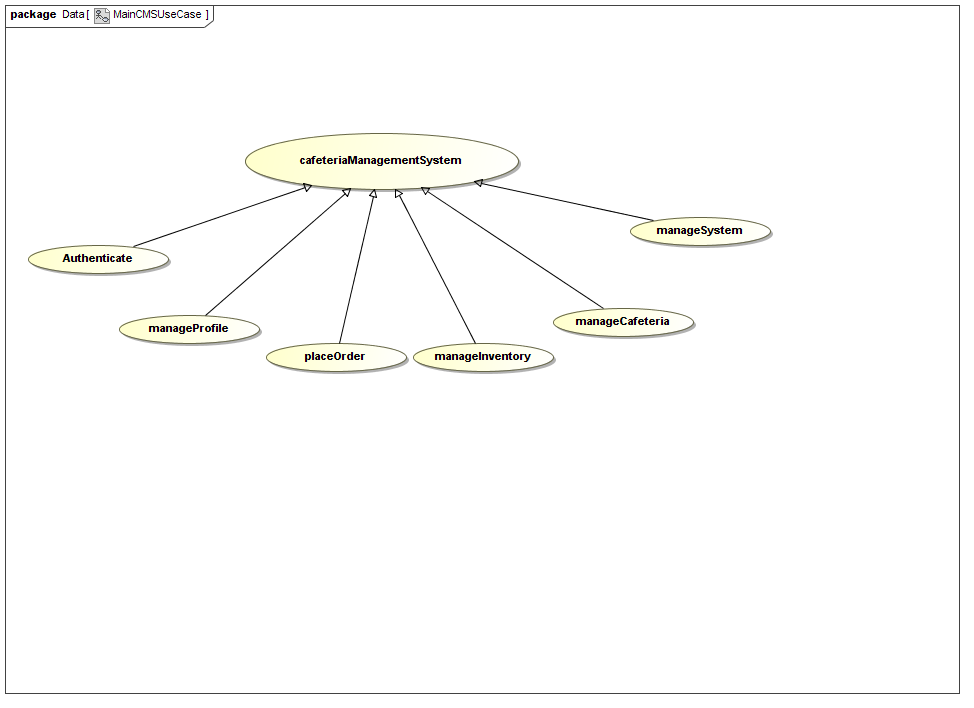
\includegraphics[width=1.0\textwidth]{../images/CMSUseCase.png}
    \caption{Cafeteria Management System Use Case} 
\end{figure}

The core of the system is a cafeteria management system that will provide functionality such as allowing users to place orders once they have registered and logged on to the system. Different types of users will have different privileges. 

%%-----AUTHENTICATION MODULE-----
\subsection{Authentication Module}

In this module, the functionality provided consists of validating the credentials entered into the system by a user whilst signing in. In addition, assistance is provided via the forgotPassword functionality. The different roles are also obtained in order to assign different functionality to users based on their roles. The register/ signup functionality is also included here. 

\begin{figure}[H]
  \centering
    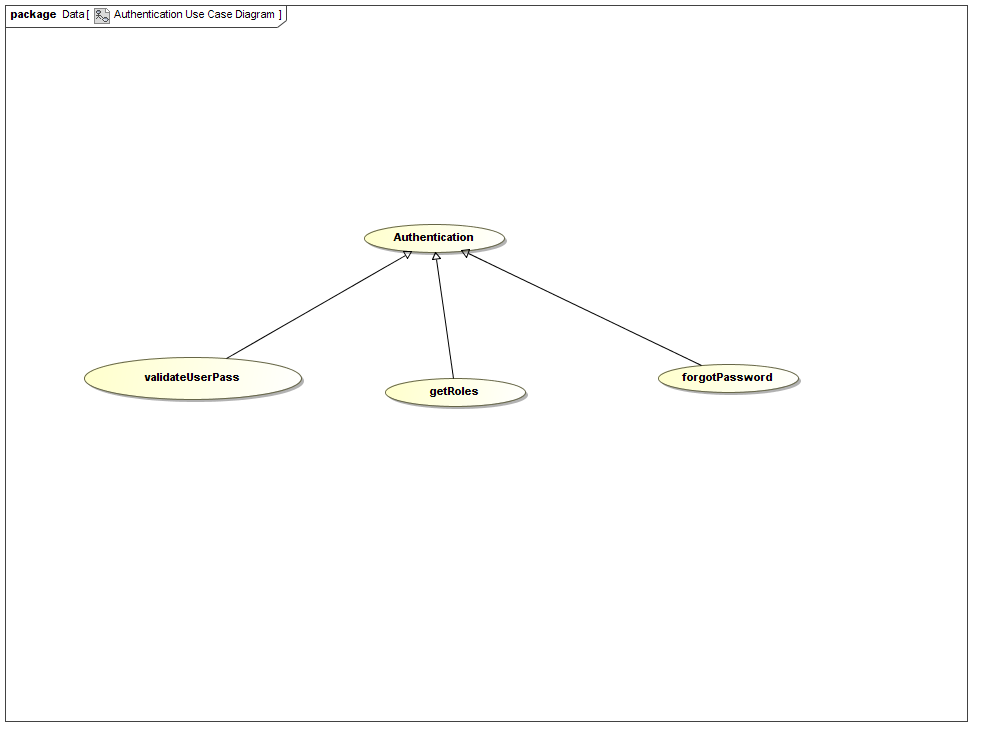
\includegraphics[width=1.0\textwidth]{../images/AuthenticationUseCaseDiagram.png}
    \caption{The main use case diagram for Authentication} 
\end{figure}

Another crutial part of the authentication module is to verify if a user may have access to certain pages given his/her role which will also contribute to the security of the data stored on our system and to control which user has access to which functionality.

\subsubsection{Forgot Password }
The service contract and activity diagram for forgotPassword follow. forgotPassword falls under the use case for Authentication (refer to page 15 - figure 12 to view this use case diagram). Here, a user who has forgotten their password will be assisted via sending an email to the user's email account with steps to follow to create a new password.
\begin{figure}[H]
  \centering
    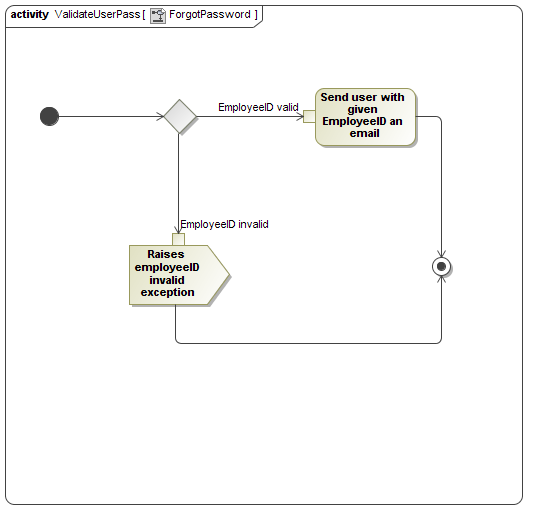
\includegraphics[width=1.0\textwidth]{../images/ForgotPasswordActivity.png}
    \caption{The activity diagram for forgotPassword} 
\end{figure}
\begin{figure}[H]
  \centering
    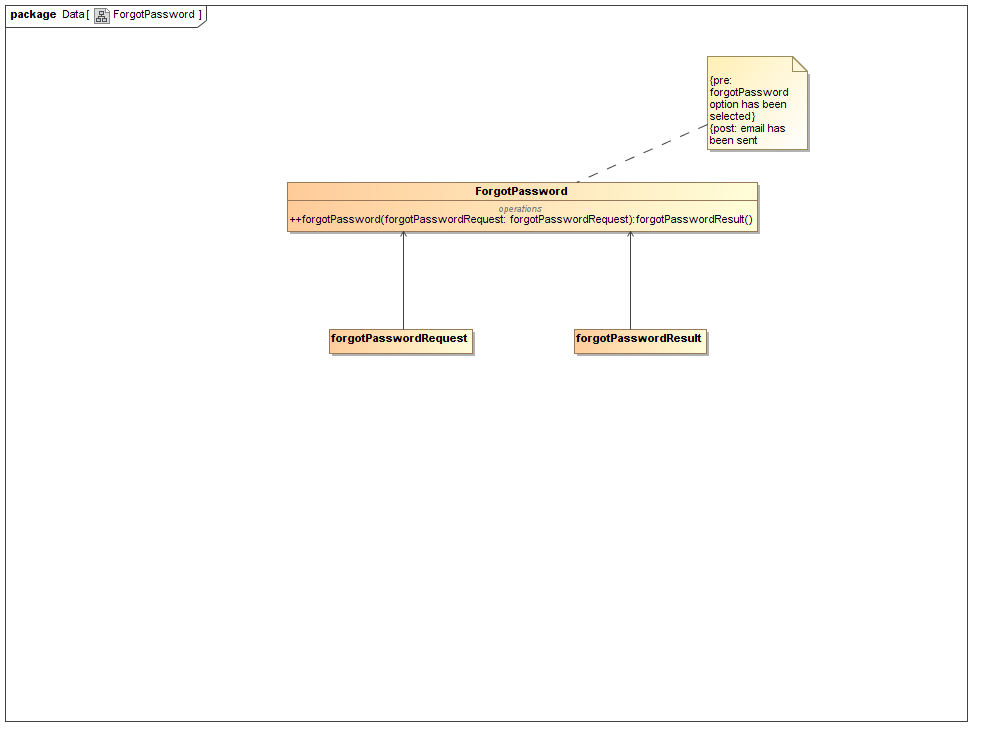
\includegraphics[width=1.0\textwidth]{../images/ForgotPassword.png}
    \caption{The service contract for forgotPassword} 
\end{figure}

\subsubsection{Validate User credentials }
The service contract and activity diagram for validateUserCredentials follow. validateUserCredentials falls under the use case for Authentication (refer to page 15 - figure 12 to view this use case diagram). Here, a user who has forgotten their password will be assisted via sending an email to the user's email account with steps to follow to create a new password.
\begin{figure}[H]
  \centering
    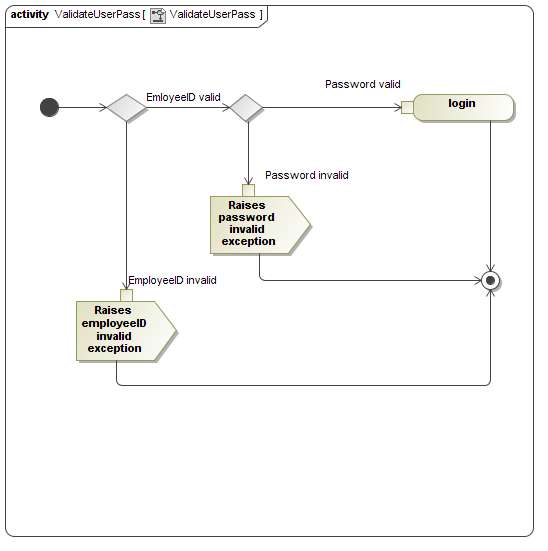
\includegraphics[width=1.0\textwidth]{../images/ValidateUserPassActivity.png}
    \caption{The activity diagram for validateUserCredentials} 
\end{figure}
\begin{figure}[H]
  \centering
    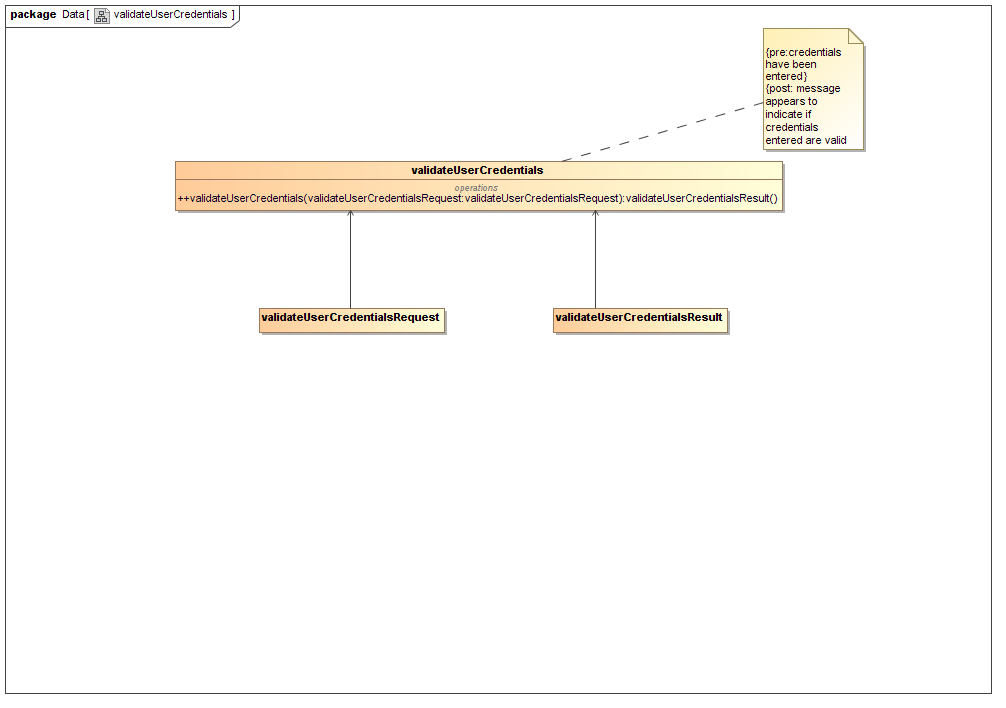
\includegraphics[width=1.0\textwidth]{../images/validateUserCredentials.png}
    \caption{The service contract for validateUserCredentials} 
\end{figure}

\subsubsection{Register }
Register provides the functionality to sign up as a user of the system. The user will set their limit, and personal details upon registration, as well as the recipient of their monthly bill. This is indicated in the following use case diagram.
\begin{figure}[H]
  \centering
    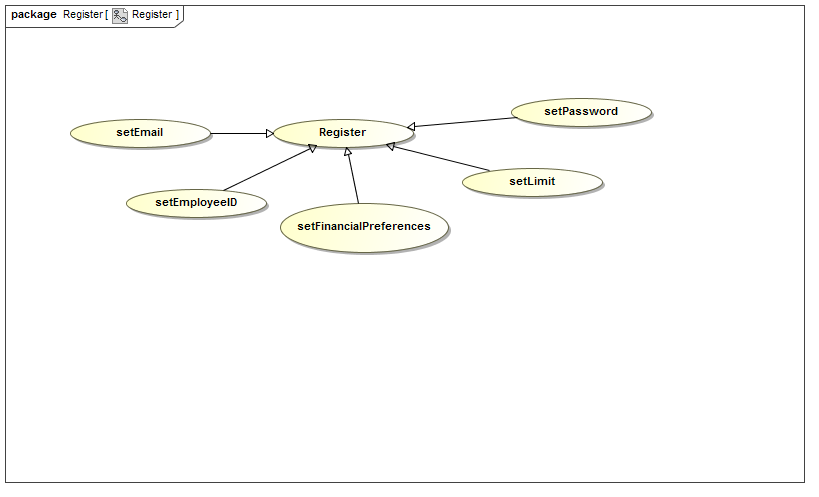
\includegraphics[width=1.0\textwidth]{../Diagrams/Register/registerUseCase.png}
    \caption{The use case for registering on the system} 
\end{figure}
\subsubsection{Set email}
The service contract and activity diagram for setEmail follow. setEmail falls under the use case for Register (refer to page   - figure  to view this use case diagram). These details, entered by the user will be stored on the system.
\begin{figure}[H]
  \centering
    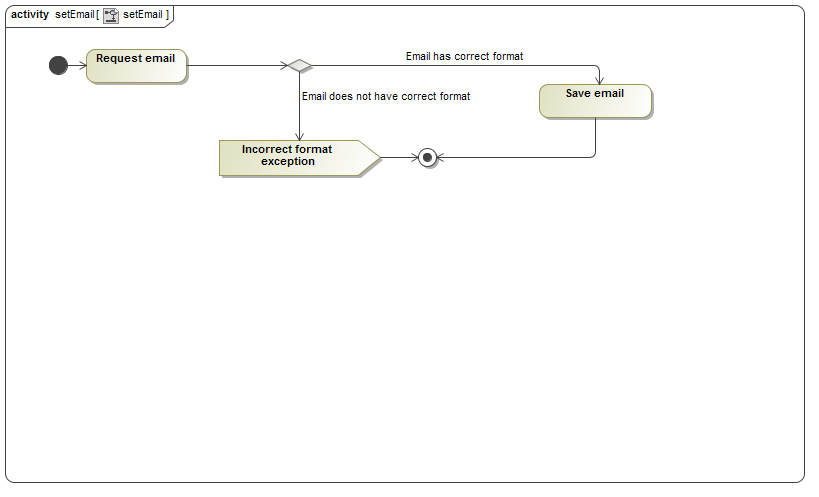
\includegraphics[width=1.0\textwidth]{../Diagrams/Register/ActivityDiagrams/setEmail1.png}
    \caption{The activity diagram for setting an email address on the system} 
\end{figure}
\begin{figure}[H]
  \centering
    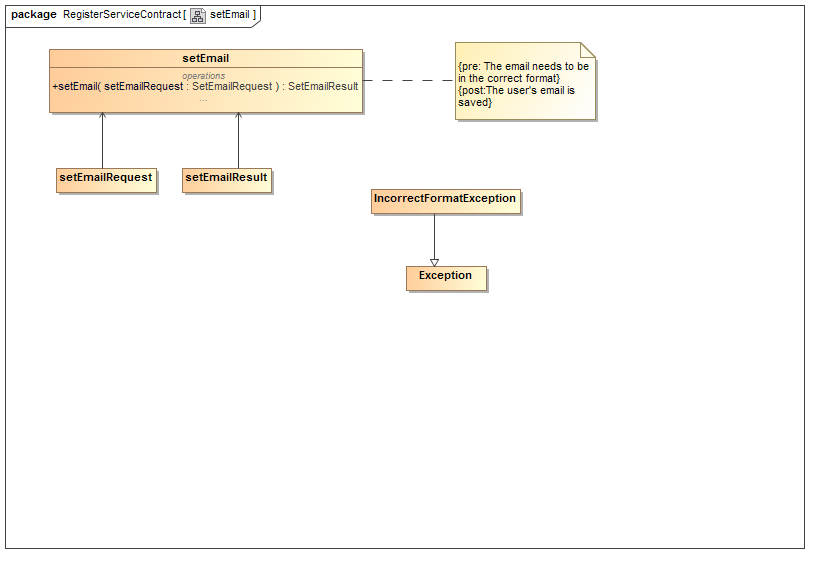
\includegraphics[width=1.0\textwidth]{../Diagrams/Register/ServiceContractsRegister/setEmailServiceContract.png}
    \caption{The service contract for setting an email address on the system} 
\end{figure}

\subsubsection{Set Password}
The service contract and activity diagram for setPassword follow. setPassword falls under the use case for Register (refer to page 8 - figure 2 to view this use case diagram). These details, entered by the user will be stored on the system.
\begin{figure}[H]
  \centering
    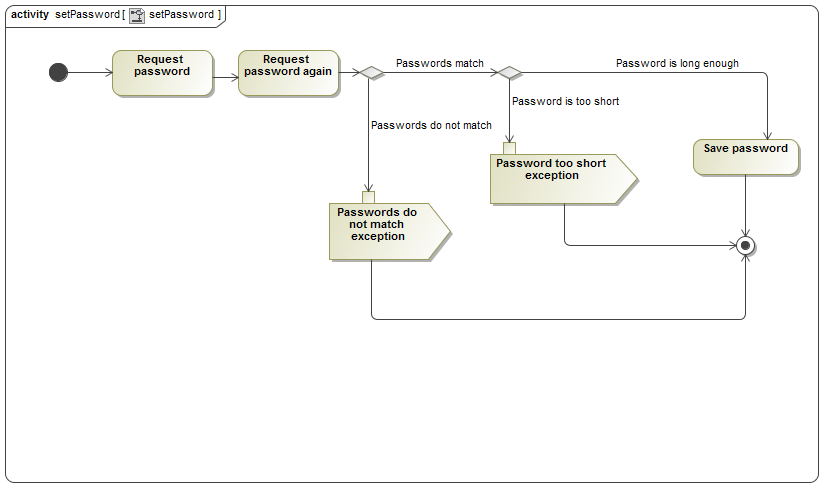
\includegraphics[width=1.0\textwidth]{../Diagrams/Register/ActivityDiagrams/setPassword1.png}
    \caption{The activity diagram for setting a password on the system} 
\end{figure}
\begin{figure}[H]
  \centering
    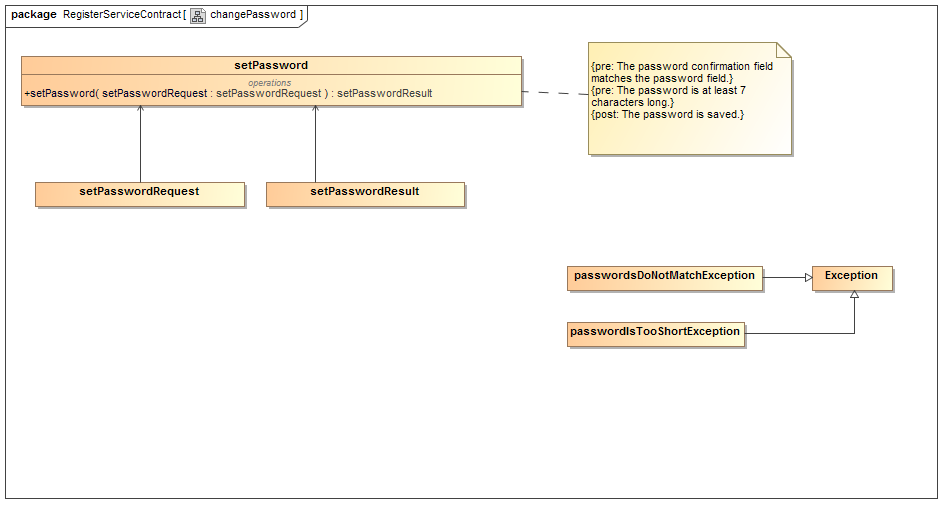
\includegraphics[width=1.0\textwidth]{../Diagrams/Register/ServiceContractsRegister/changePasswordServiceContract.png}
    \caption{The service contract for setting a password on the system} 
\end{figure}

\subsubsection{Set Limit}
The service contract and activity diagram for setLimit follow. setLimit falls under the use case for Register (refer to page 8 - figure 2 to view this use case diagram). These details, entered by the user will be stored on the system. 
\begin{figure}[H]
  \centering
    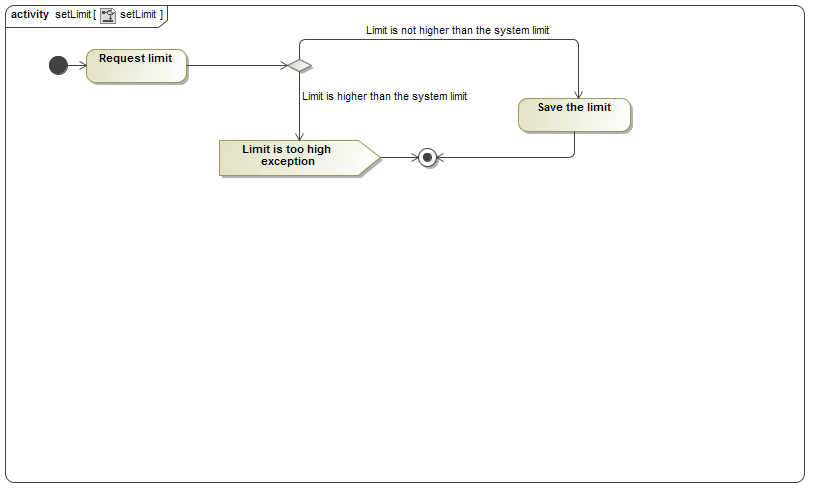
\includegraphics[width=1.0\textwidth]{../Diagrams/Register/ActivityDiagrams/setLimit.png}
    \caption{The activity diagram for setting a limit on the system} 
\end{figure}
\begin{figure}[H]
  \centering
    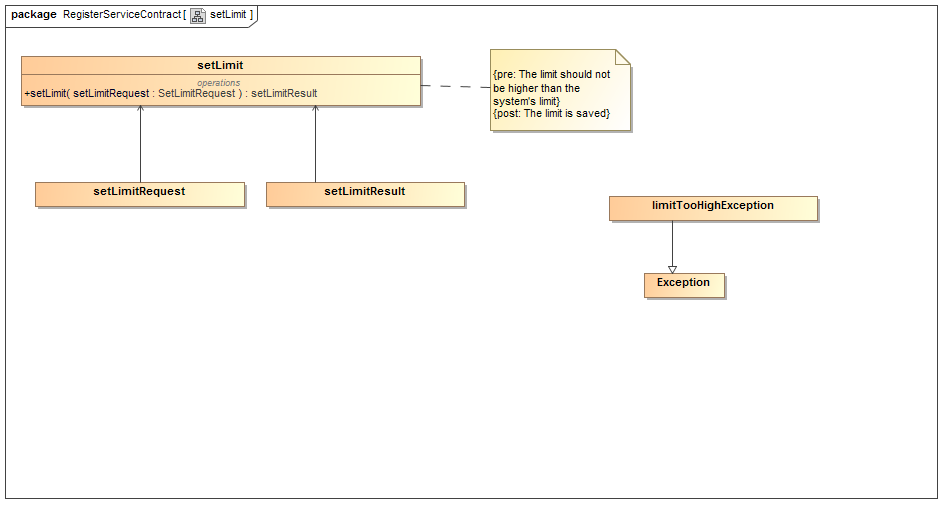
\includegraphics[width=1.0\textwidth]{../Diagrams/Register/ServiceContractsRegister/setLimit.png}
    \caption{The service contract for setting a limit on the system} 
\end{figure}

\subsubsection{Set Employee ID }
The service contract and activity diagram for setEmployeeID follow. setEmployeeID falls under the use case for Register (refer to page 8 - figure 2 to view this use case diagram). These details, entered by the user will be stored on the system.
\begin{figure}[H]
  \centering
    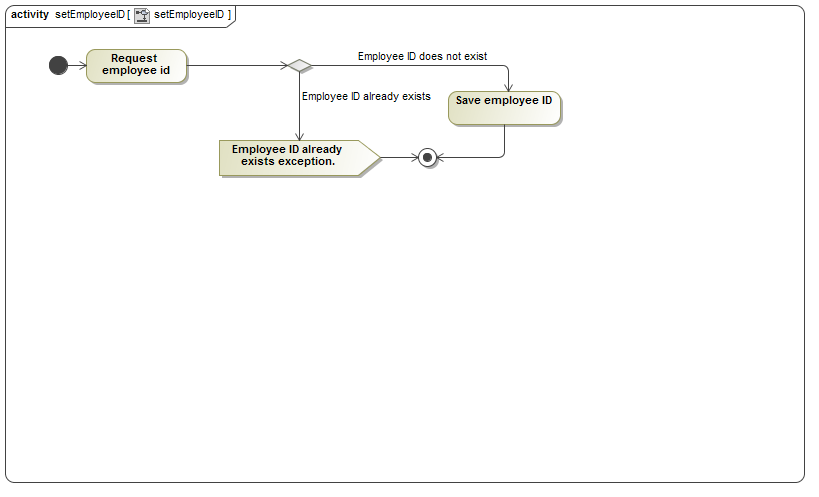
\includegraphics[width=1.0\textwidth]{../Diagrams/Register/ActivityDiagrams/setEmployeeID1.png}
    \caption{The activity diagram for setting an employeeId on the system} 
\end{figure}
\begin{figure}[H]
  \centering
    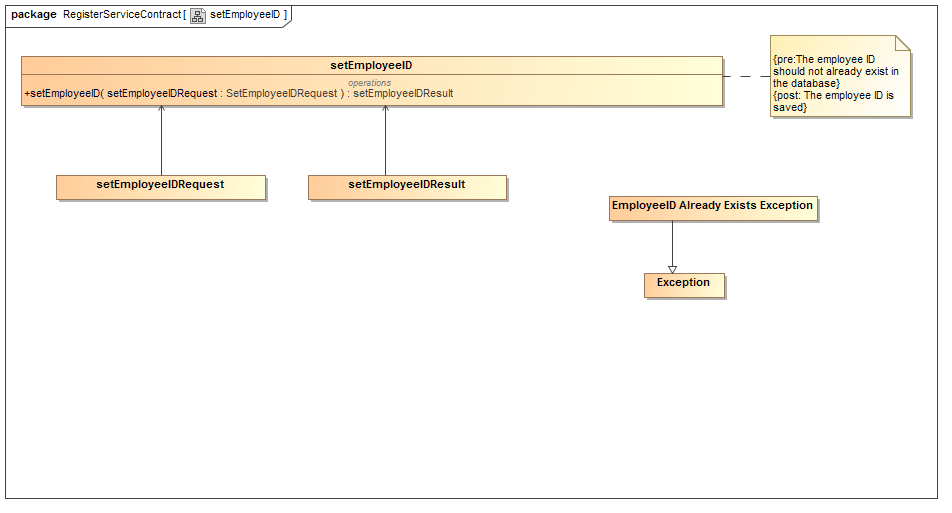
\includegraphics[width=1.0\textwidth]{../Diagrams/Register/ServiceContractsRegister/setEmployeeIDServiceContract.png}
    \caption{The service contract for setting an employeeId on the system} 
\end{figure}

\subsubsection{Set Financial Preferences }
The service contract and activity diagram for setFinancialPreferences follow. setFinancialPreferences falls under the use case for Register (refer to page 8 - figure 2 to view this use case diagram). These details, entered by the user will be stored on the system.
\begin{figure}[H]
  \centering
    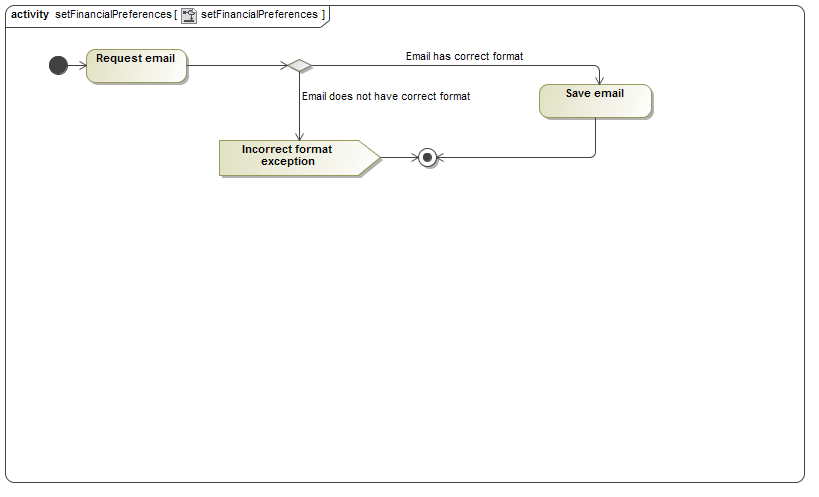
\includegraphics[width=1.0\textwidth]{../Diagrams/Register/ActivityDiagrams/setFinancialPreferences1.png}
    \caption{The activity diagram for setting financial preferences on the system} 
\end{figure}
\begin{figure}[H]
  \centering
    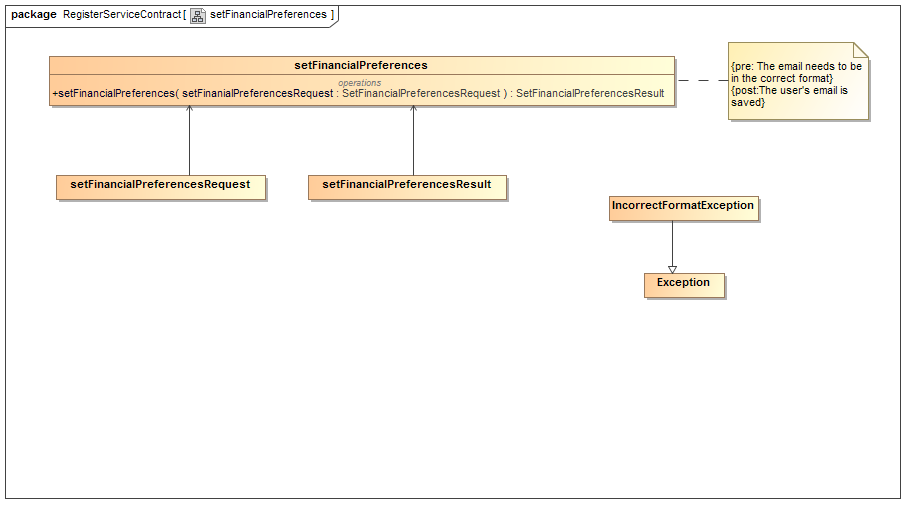
\includegraphics[width=1.0\textwidth]{../Diagrams/Register/ServiceContractsRegister/setFinancialPreferencesServiceContract.png}
    \caption{The service contract for setting financial preferences on the system} 
\end{figure}

%%---------MANAGE CAFETERIA MODULE-----
\subsection{Manage Cafeteria Module}

The menu module consists of the functionality of adding and removing menu items from the menu from which the user will place orders. This use case diagram indicates the functionality that this module consists of such as addMenuItem, updateMenuItem, searchMenuItem and deleteMenuItem, which are the use cases of this module.

\begin{figure}[H]
  \centering
    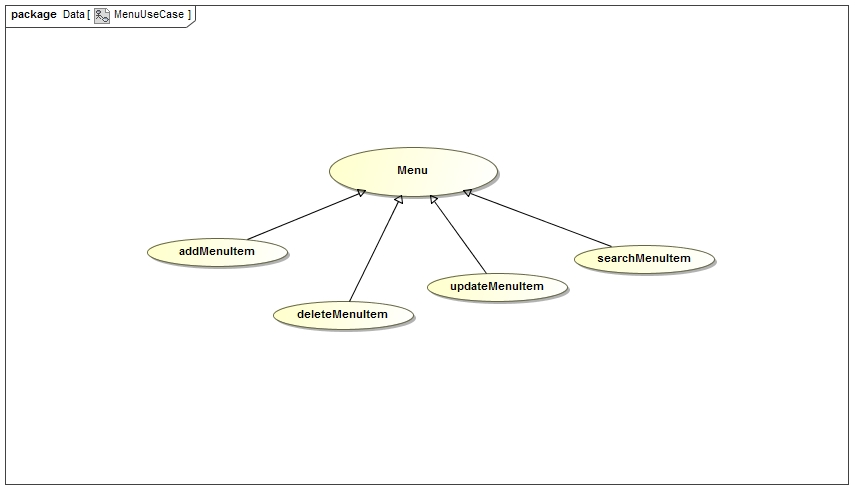
\includegraphics[width=1.0\textwidth]{../images/MenuUseCase.jpg}
    \caption{The use case for menu} 
\end{figure}

 \subsubsection{addMenuItem}
The service contract and activity diagram for addMenuItem follow. addMenuItem falls under the use case for Menu (refer to page   - figure   to view this use case diagram). The system allows the cafeteria manager to add items to the menu via the menu managing page.
\begin{figure}[H]
  \centering
    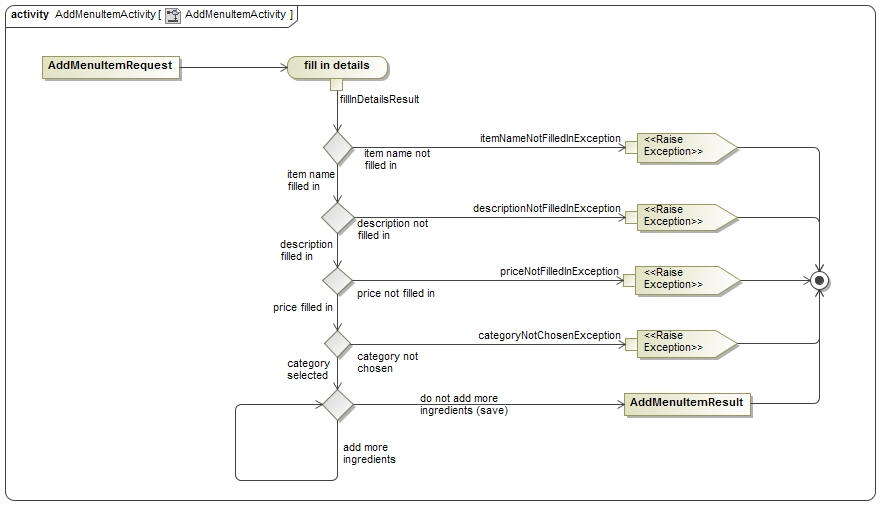
\includegraphics[width=1.0\textwidth]{../images/AddMenuItemActivity.jpg}
    \caption{The activity diagram for adding a menu item } 
\end{figure}
\begin{figure}[H]
	\centering
	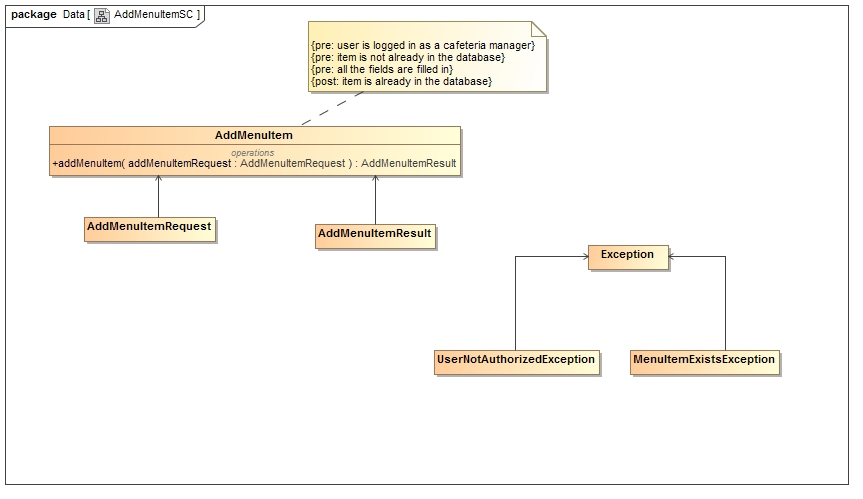
\includegraphics[width=1.0\textwidth]{../images/AddMenuItemSC.jpg}
	\caption{The service contract for adding a menu item}
\end{figure}

 \subsubsection{deleteMenuItem}
The service contract and activity diagram for deleteMenuItem follow. deleteMenuItem falls under the use case for Menu (refer to page   - figure   to view this use case diagram). The system allows the cafeteria manager to delete items from the menu via the menu managing page.
\begin{figure}[H]
  \centering
    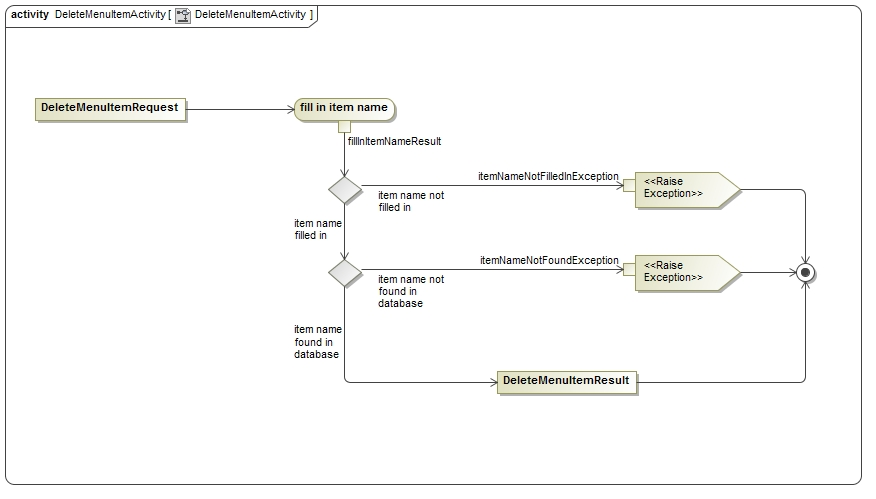
\includegraphics[width=1.0\textwidth]{../images/DeleteMenuItemActivity.jpg}
    \caption{The activity diagram for deleting a menu item } 
\end{figure}
\begin{figure}[H]
	\centering
	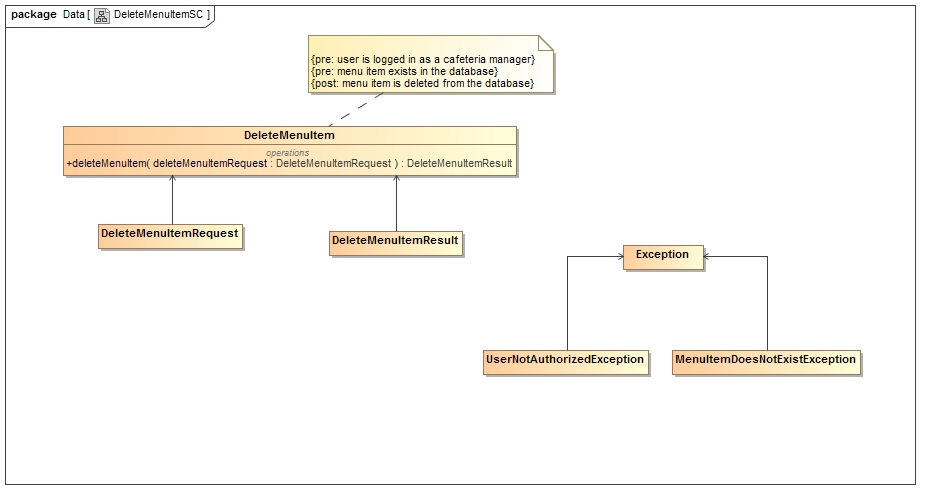
\includegraphics[width=1.0\textwidth]{../images/DeleteMenuItemSC.jpg}
	\caption{The service contract for deleting a menu item}
\end{figure}

 \subsubsection{searchMenuItem}
The service contract and activity diagram for searchMenuItem follow. searchMenuItem falls under the use case for Menu (refer to page   - figure   to view this use case diagram). The system allows the cafeteria manager to search for items from the menu via the menu managing page.
\begin{figure}[H]
  \centering
    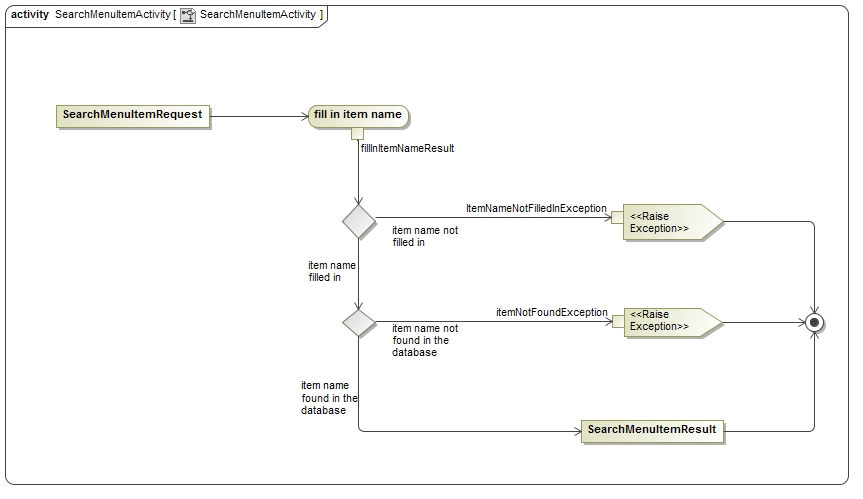
\includegraphics[width=1.0\textwidth]{../images/SearchMenuItemActivity.jpg}
    \caption{The activity diagram for searching for a menu item } 
\end{figure}
\begin{figure}[H]
	\centering
	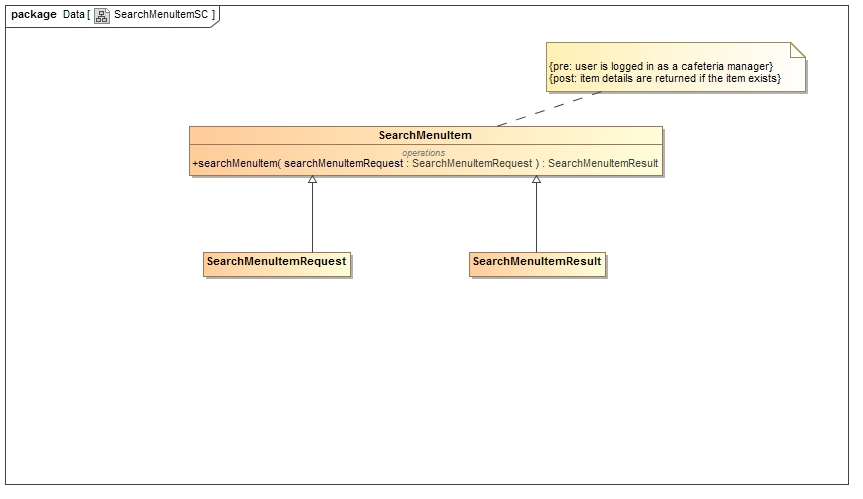
\includegraphics[width=1.0\textwidth]{../images/SearchMenuItemSC.jpg}
	\caption{The service contract for searching for a menu item}
\end{figure}

 \subsubsection{updateMenuItem}
The service contract and activity diagram for updateMenuItem follow. updateMenuItem falls under the use case for Menu (refer to page   - figure   to view this use case diagram). The system allows the cafeteria manager to update menu items' unit, quantity and name via the menu managing page.
\begin{figure}[H]
  \centering
    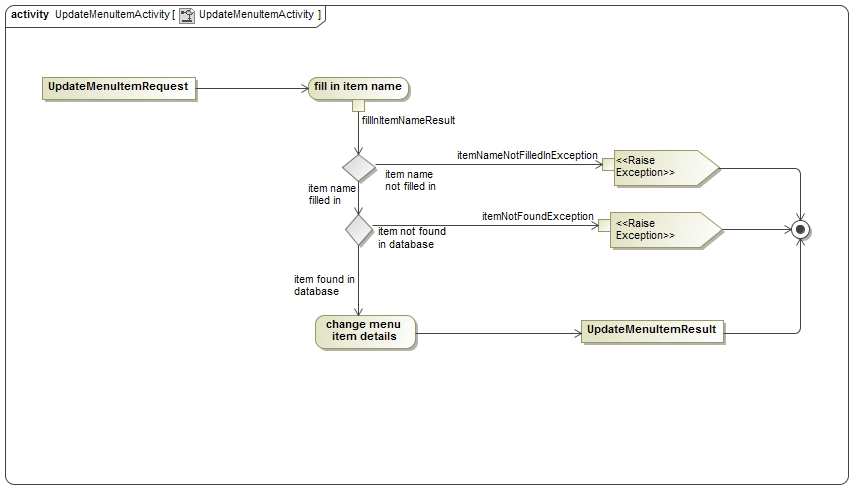
\includegraphics[width=1.0\textwidth]{../images/UpdateMenuItemActivity.jpg}
    \caption{The activity diagram for updating a menu item } 
\end{figure}
\begin{figure}[H]
	\centering
	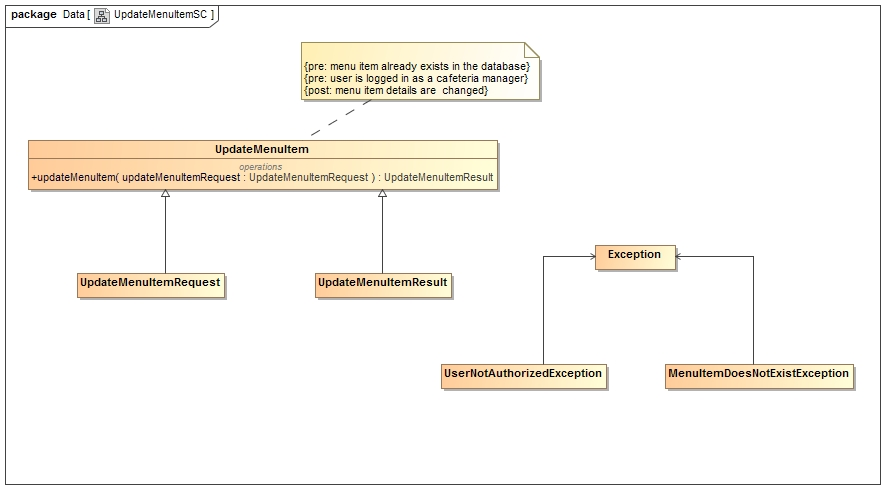
\includegraphics[width=1.0\textwidth]{../images/UpdateMenuItemSC.jpg}
	\caption{The service contract for updating a menu item}
\end{figure}

%%-----PLACE ORDERS MODULE-----
\subsection{Place Orders Module}

The main functionality the system serves to provide, is  to allow the user to use their access card number to purchase food items from the cafeteria via the system. This use case diagram indicates the functionality around placing orders, such as CheckProductAvailability and checkLimits, which are the use cases of this module.

\begin{figure}[H]
  \centering
    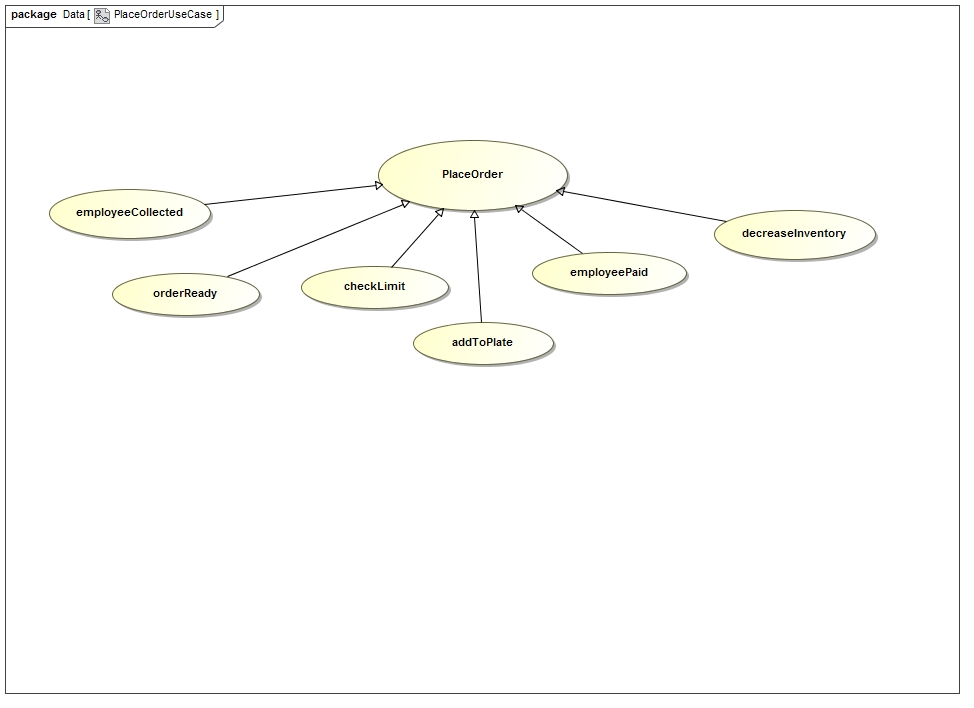
\includegraphics[width=1.0\textwidth]{../images/PlaceOrderUseCase.jpg}
    \caption{The use case for placing an order} 
\end{figure}
 
\subsubsection{CheckProductAvailability}
The service contract and activity diagram for CheckProductAvailability follow. CheckProductAvailability falls under the use case for Place Orders (refer to page 27 - figure 27 to view this use case diagram). The system will check whether the product that the user has selected to purchase is currently in stock.
\begin{figure}[H]
  \centering
    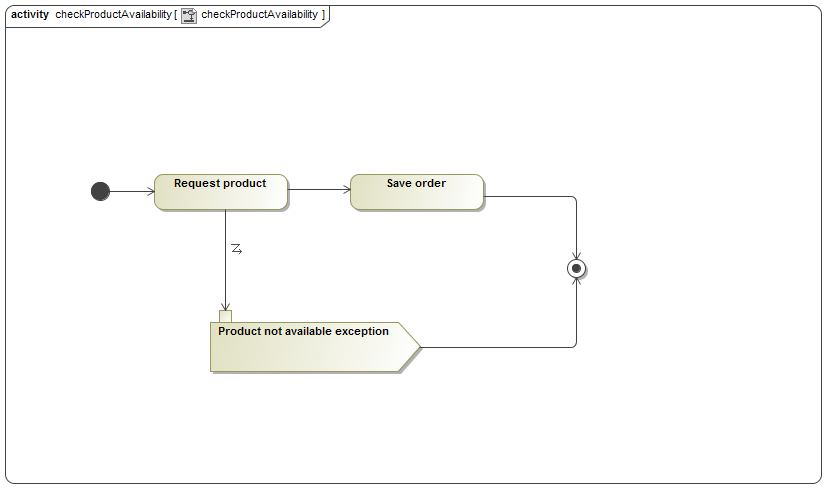
\includegraphics[width=1.0\textwidth]{../images/checkProductAvailability.png}
    \caption{The activity diagram for checking product availability } 
\end{figure}
 
\begin{figure}[H]
	\centering
	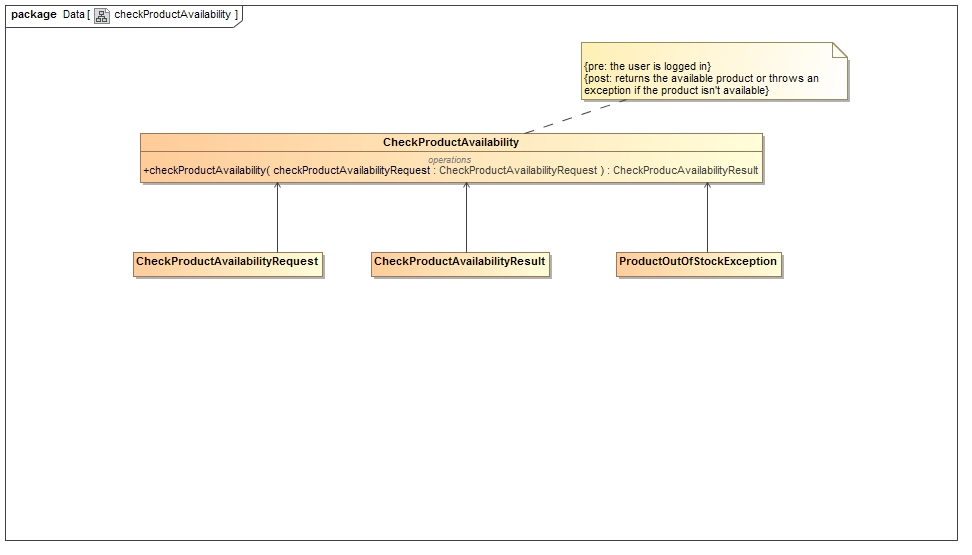
\includegraphics[width=1.0\textwidth]{../images/checkProductAvailabilitySC.jpg}
	\caption{The service contract for checking product availability}
\end{figure}

\subsubsection{markAsReady}
The service contract and activity diagram for markAsReady follow. markAsReady falls under the use case for Place Orders (refer to page 27 - figure 27 to view this use case diagram). The cashier will be the only user with access to this functionality and when the order is marked as ready, the status of the order in the model is changed to ready. This will also send an email notification to the user that their order is ready for collection. 
\begin{figure}[H]
  \centering
    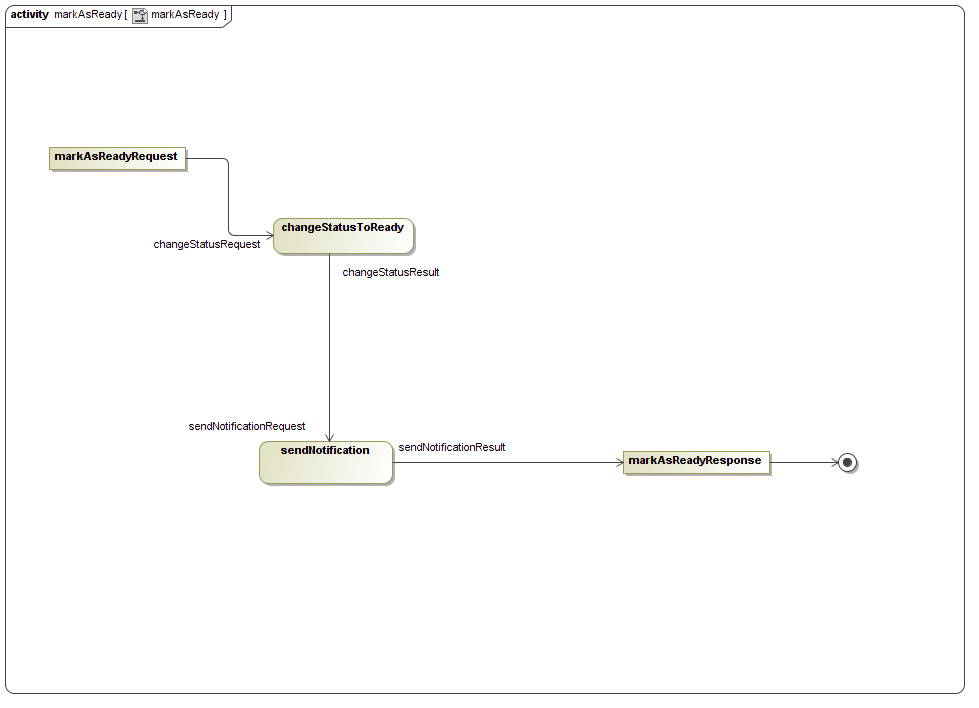
\includegraphics[width=1.0\textwidth]{../images/markAsReadyActivity.png}
    \caption{The activity diagram for marking an order as ready } 
\end{figure}
 
\begin{figure}[H]
	\centering
	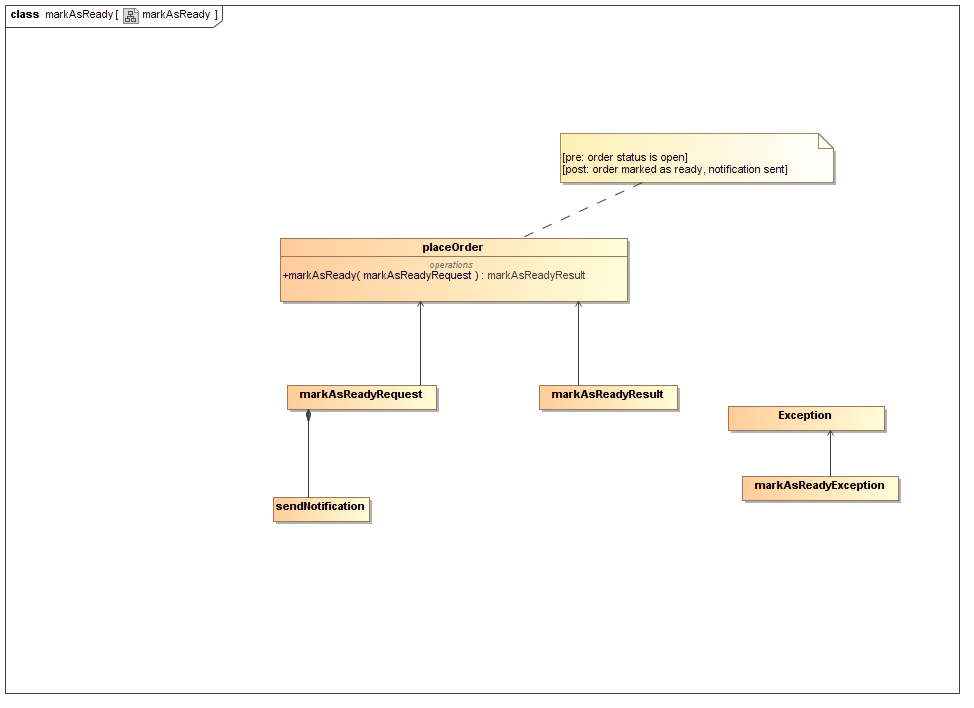
\includegraphics[width=1.0\textwidth]{../images/markAsReadySC.png}
	\caption{The service contract for marking an order as ready}
\end{figure}

\subsubsection{addToPlate }
The service contract and activity diagram for addToPlate follow. addToPlate falls under the use case for PlaceOrder (refer to page 27- figure 27 to view this use case diagram). This is where a user can select items from the menu and save them on their plate via the addToPlate button. The user can then view these via the "On my plate" page and can also edit these.
\begin{figure}[H]
  \centering
    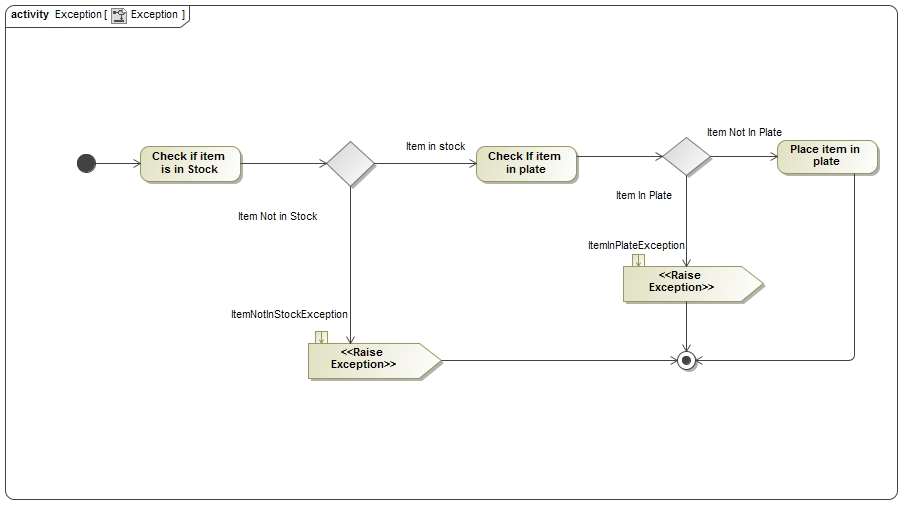
\includegraphics[width=1.0\textwidth]{../images/AddToPlateActivity.jpg}
    \caption{The activity diagram for adding a menu item to plate} 
\end{figure}
\begin{figure}[H]
  \centering
    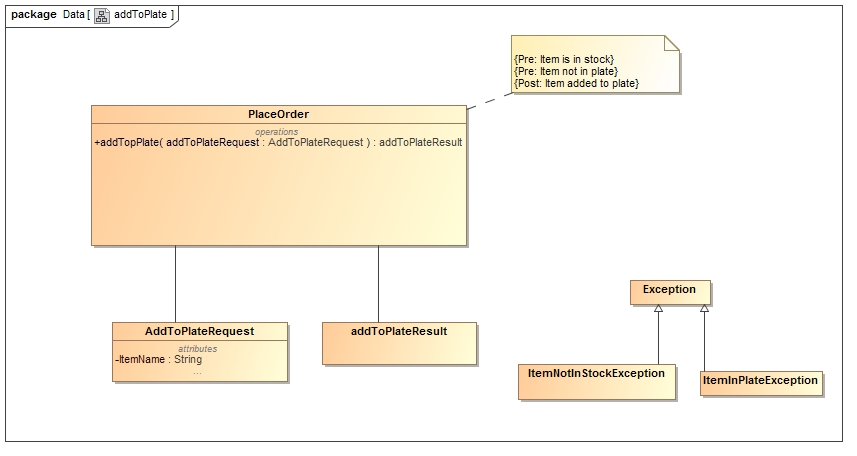
\includegraphics[width=1.0\textwidth]{../images/addToPlateServicee.jpg}
    \caption{The service contract for adding a menu item to plate} 
\end{figure}

\subsubsection{markAsCollected}
The service contract and activity diagram for markAsCollected follow. markAsCollected falls under the use case for Place Orders (refer to page 27 - figure 27 to view this use case diagram). The cashier will be the only user with access to this functionality and when the order is marked as collected, the status of the order in the model is changed to closed. It is important to note that by marking it as just merely "collected", the system will know to deduct the amount from the user's monthly balance, as the user has not paid with cash. This hence marks that the order has collected their order and their order has been processed. It will then no longer be displayed on the cashiers page.
\begin{figure}[H]
  \centering
    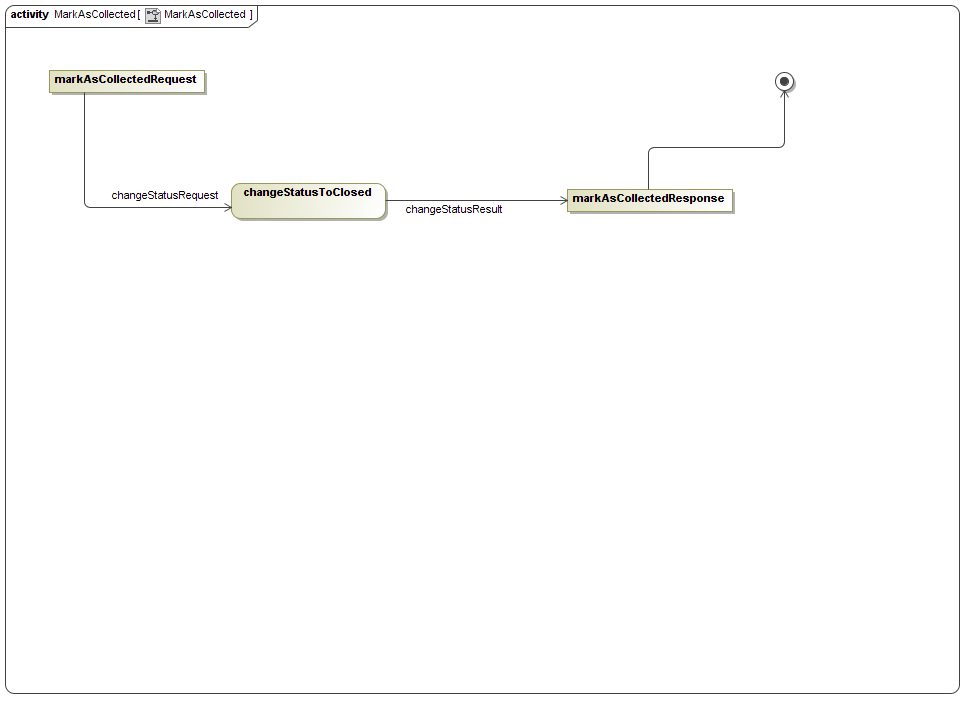
\includegraphics[width=1.0\textwidth]{../images/MarkAsCollectedActivity.png}
    \caption{The activity diagram for marking an order as collected } 
\end{figure}
 
\begin{figure}[H]
	\centering
	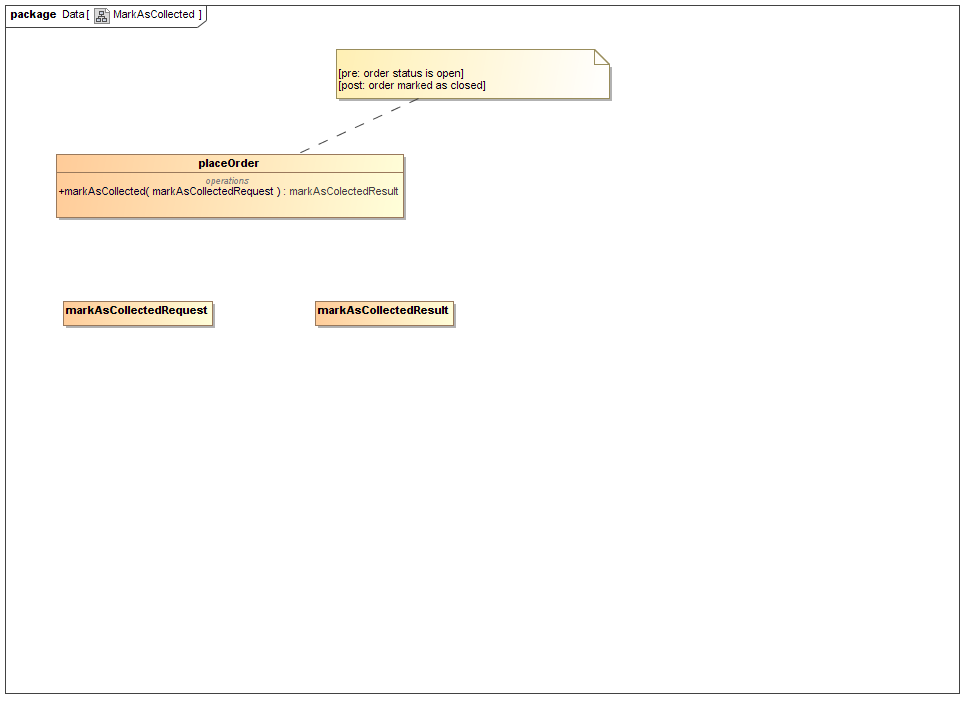
\includegraphics[width=1.0\textwidth]{../images/MarkAsCollectedSC.png}
	\caption{The service contract for marking an order as collected}
\end{figure}


\subsubsection{checkLimit}
The service contract and activity diagram for checkLimit follow. checkLimit falls under the use case for Place Orders (refer to figure 27 page 27 to view this use case diagram). The system will be able to view the user's personal limit to make sure that the total of the bill is not larger than the users spending limit. 
\begin{figure}[H]
  \centering
    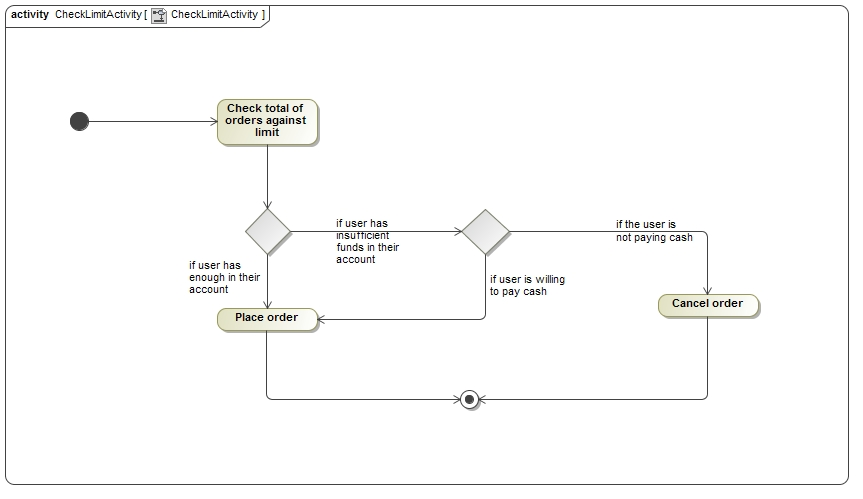
\includegraphics[width=1.0\textwidth]{../images/CheckLimitActivity.jpg}
    \caption{The activity diagram for checking limits} 
\end{figure}

\begin{figure}[H]
	\centering
	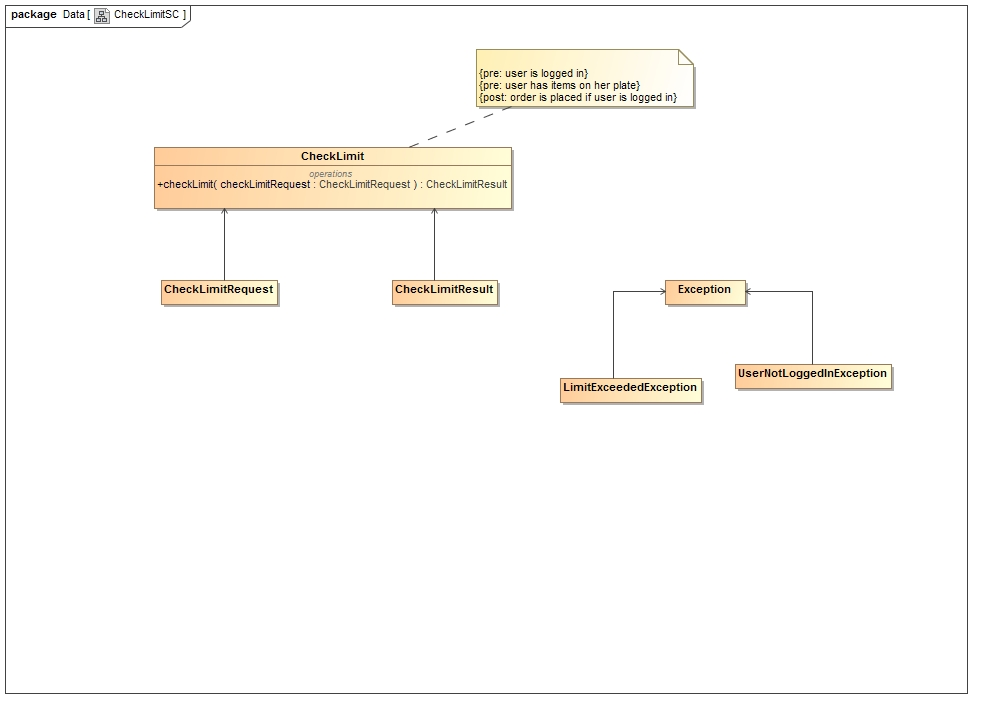
\includegraphics[width=1.0\textwidth]{../images/CheckLimitSC.jpg}
	\caption{The service contract for checking limits}
\end{figure}

\subsubsection{employeePaid}
The service contract and activity diagram for employeePaid follow. employeePaid falls under the use case for Place Orders (refer to figure 27 page 27 to view this use case diagram). The cashier will be able to check this off if the client pays using cash instead of paying from their account. This will ensure that money isn't deducted from the user's limit because they paid cash. 
\begin{figure}[H]
  \centering
    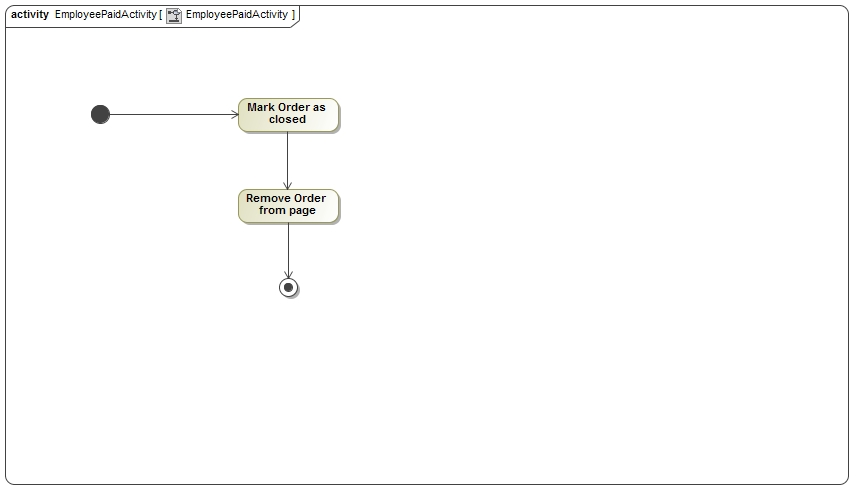
\includegraphics[width=1.0\textwidth]{../images/EmployeePaidActivity.jpg}
    \caption{The activity diagram for employee paid} 
\end{figure}

\begin{figure}[H]
	\centering
	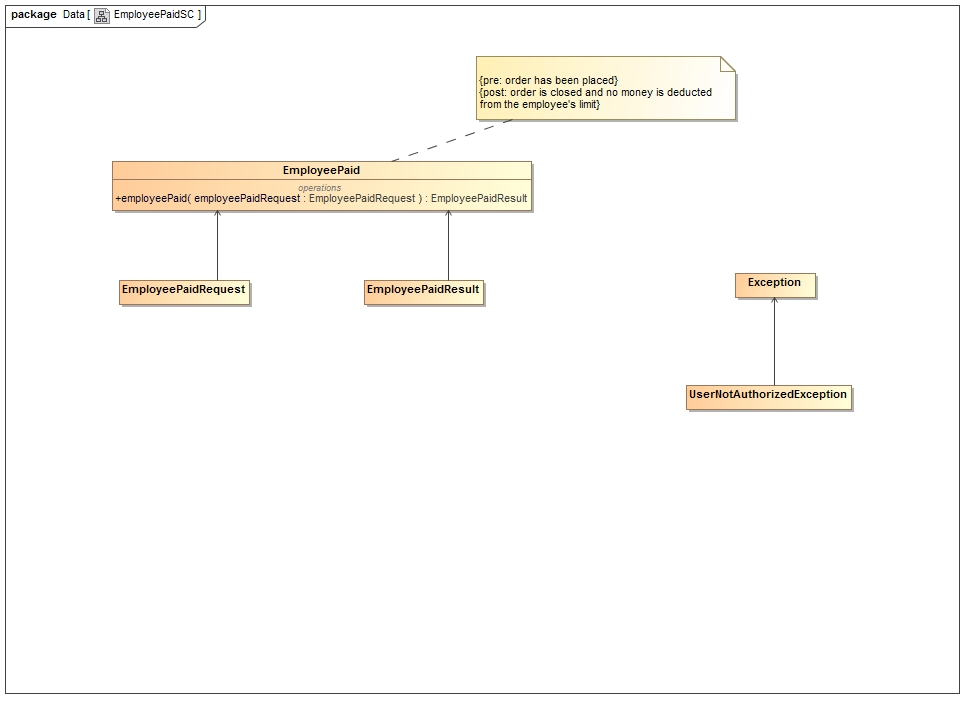
\includegraphics[width=1.0\textwidth]{../images/EmployeePaidSC.jpg}
	\caption{The service contract for employee paid}
\end{figure}

%%-----MANAGE INVENTORY MODULE-----
\subsection{Manage Inventory Module}

The inventory module is where the cafeteria manager will keep track of stock additions and removals. Different menu items require certain inventory items.This use case diagram indicates the functionality around adding, deleting, searching for and updating inventory.

\begin{figure}[H]
  \centering
    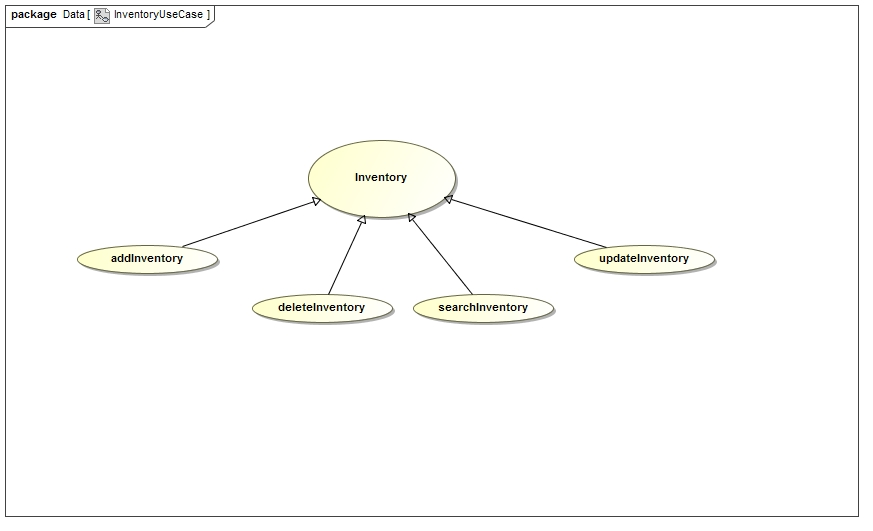
\includegraphics[width=1.0\textwidth]{../images/InventoryUseCase.jpg}
    \caption{The use case for inventory} 
\end{figure}

\subsubsection{addInventory}
The service contract and activity diagram for addInventory to follow. addInventory falls under the use case for Inventory (refer to page   figure   to view this use case diagram). The cafeteria manager will be able to manage inventory items via the allocated page.
\begin{figure}[H]
  \centering
    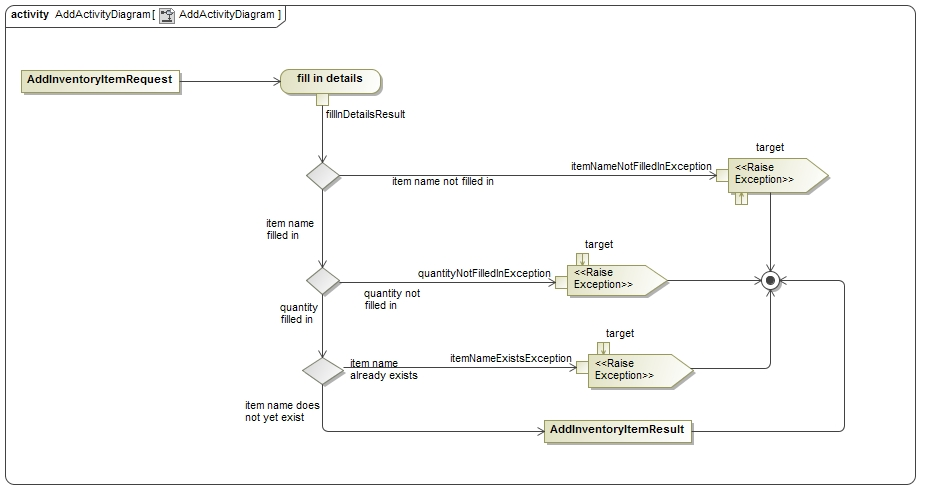
\includegraphics[width=1.0\textwidth]{../images/AddActivityDiagram.jpg}
    \caption{The activity diagram for adding inventory} 
\end{figure}

\begin{figure}[H]
	\centering
	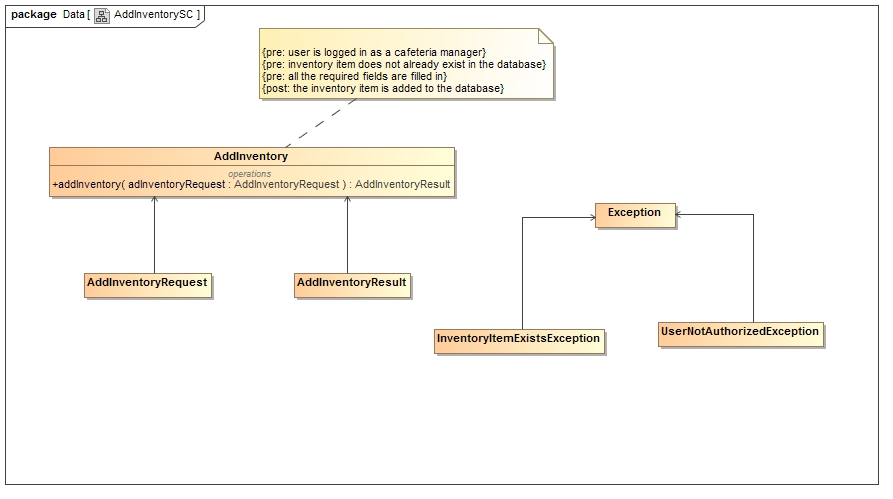
\includegraphics[width=1.0\textwidth]{../images/AddInventorySC.jpg}
	\caption{The service contract for adding inventory}
\end{figure}

\subsubsection{searchInventory}
The service contract and activity diagram for searchInventory to follow. searchInventory falls under the use case for Inventory (refer to page   figure   to view this use case diagram). The cafeteria manager will be able to search for inventory items via the allocated page and from there be able to delete or update them.
\begin{figure}[H]
  \centering
    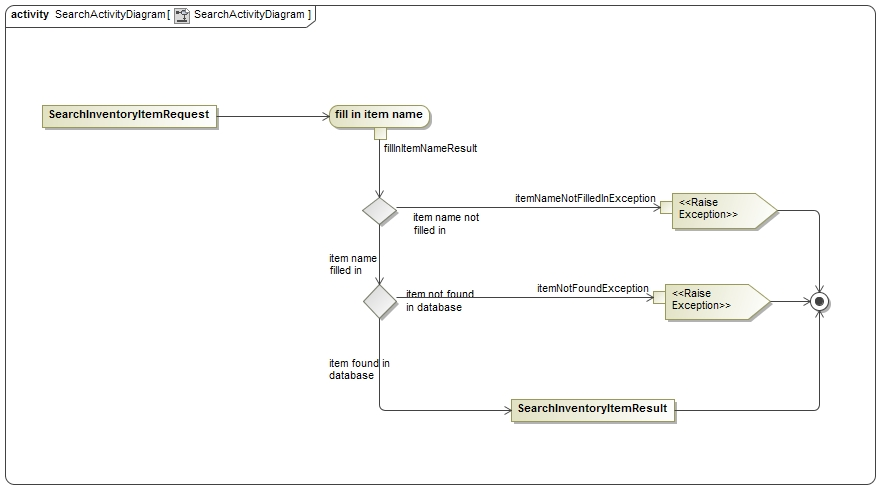
\includegraphics[width=1.0\textwidth]{../images/SearchActivityDiagram.jpg}
    \caption{The activity diagram for searching for inventory} 
\end{figure}

\begin{figure}[H]
	\centering
	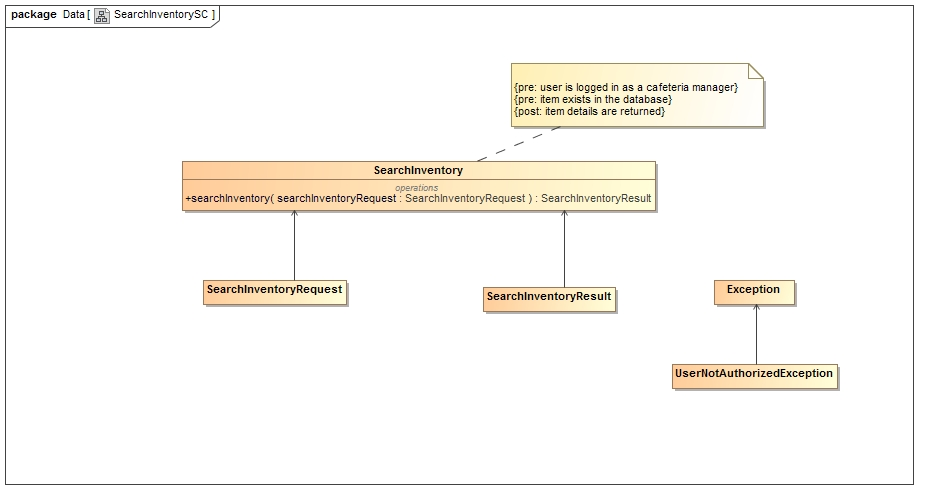
\includegraphics[width=1.0\textwidth]{../images/SearchInventorySC.jpg}
	\caption{The service contract for searching for inventory}
\end{figure}

\subsubsection{deleteInventory}
The service contract and activity diagram for deleteInventory to follow. deleteInventory falls under the use case for Inventory (refer to page   figure   to view this use case diagram). The cafeteria manager will be able to delete inventory items via the allocated page.
\begin{figure}[H]
  \centering
    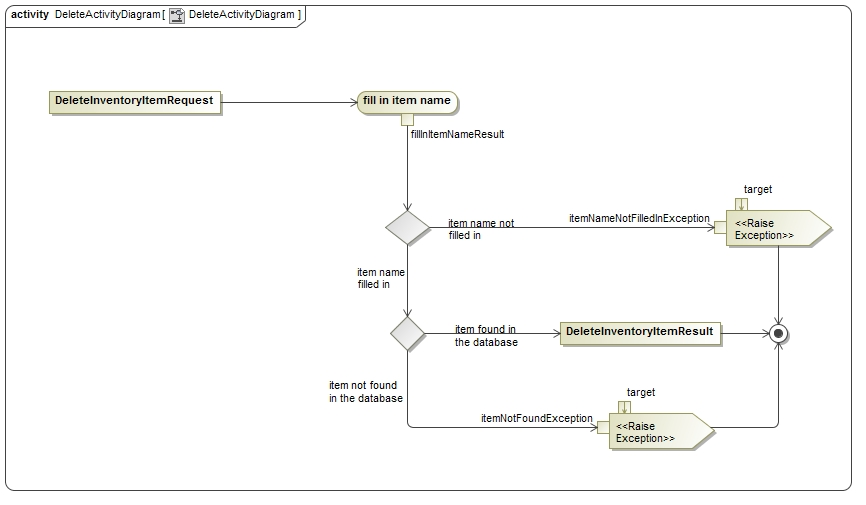
\includegraphics[width=1.0\textwidth]{../images/DeleteActivityDiagram.jpg}
    \caption{The activity diagram for adding inventory} 
\end{figure}

\begin{figure}[H]
	\centering
	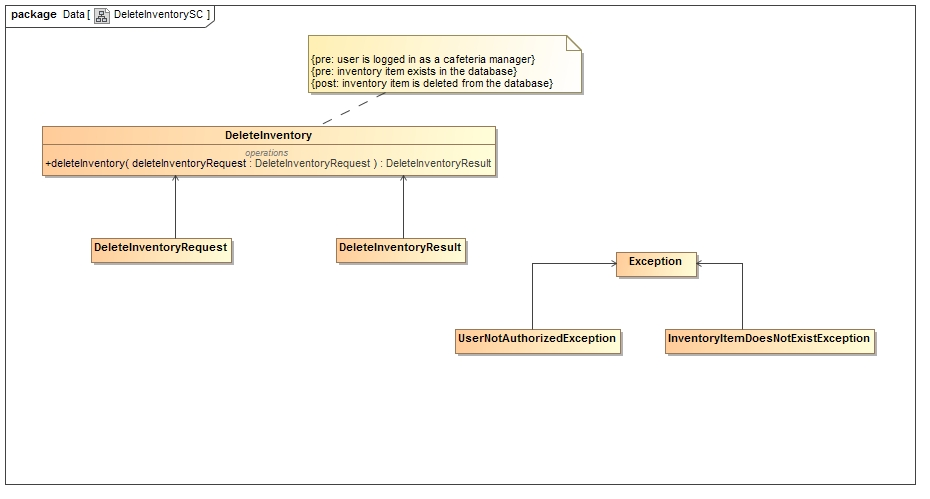
\includegraphics[width=1.0\textwidth]{../images/DeleteInventorySC.jpg}
	\caption{The service contract for adding inventory}
\end{figure}

\subsubsection{updateInventory}
The service contract and activity diagram for updateInventory to follow. updateInventory falls under the use case for Inventory (refer to page   figure   to view this use case diagram). The cafeteria manager will be able to update inventory items via the allocated page.
\begin{figure}[H]
  \centering
    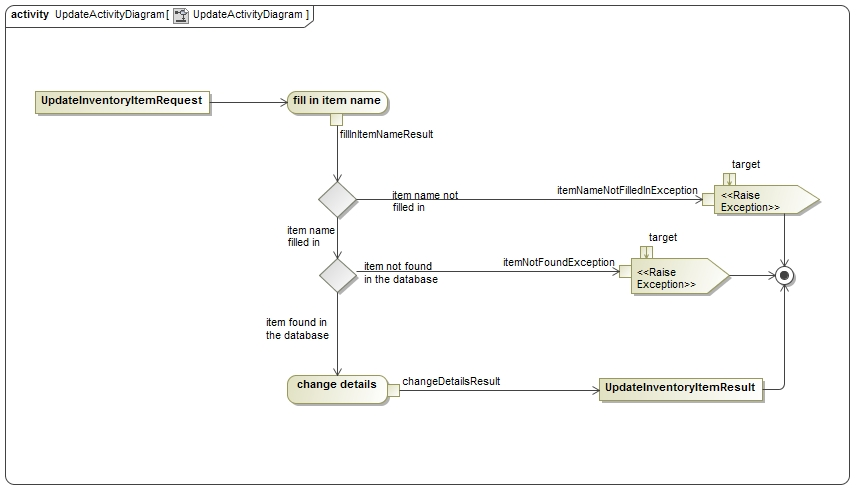
\includegraphics[width=1.0\textwidth]{../images/UpdateActivityDiagram.jpg}
    \caption{The activity diagram for updating inventory} 
\end{figure}

\begin{figure}[H]
	\centering
	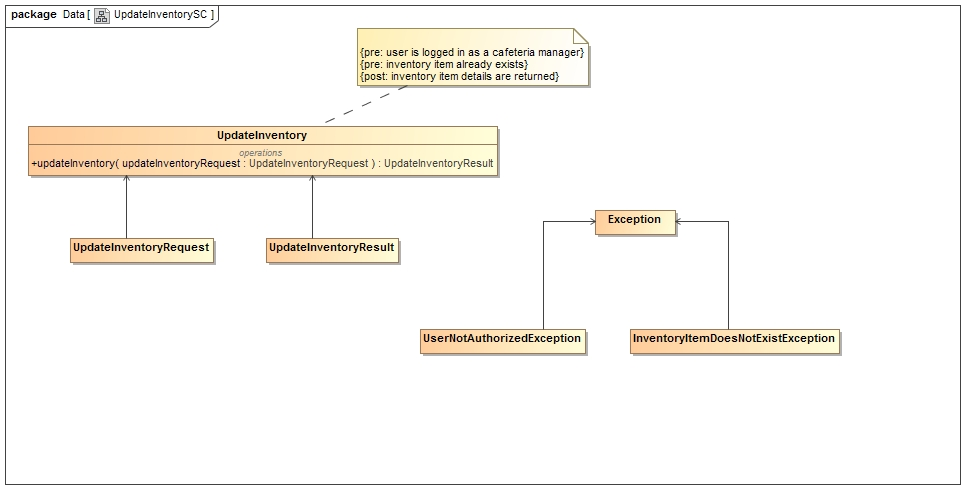
\includegraphics[width=1.0\textwidth]{../images/UpdateInventorySC.jpg}
	\caption{The service contract for updating inventory}
\end{figure}

%%-----Manage Profile module-----
\subsection{Manage Profile Module}
 The user will be allowed to customize various settings such as resetting his/her personal limit, changing password and email, displaying the bill and viewing favourites. The following use case diagram indicates the above mentioned functionality around managing the profile. Hence, it has the use cases generateFavourite and edit profile.

\begin{figure}[H]
  \centering
    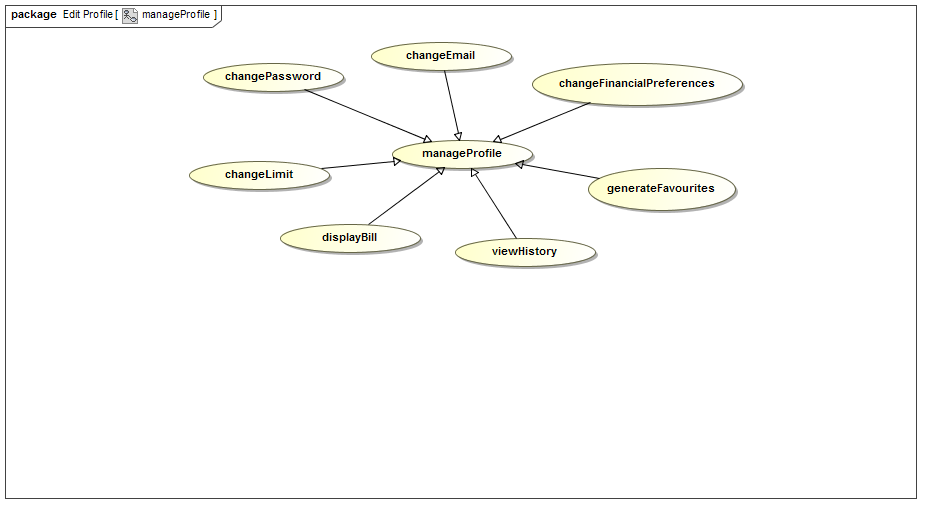
\includegraphics[width=1.0\textwidth]{../Diagrams/ManageProfile/manageProfileUseCase.png}
    \caption{The use case diagram for managing profile} 
\end{figure}

\subsubsection{setFinancialPreferences}
The service contract and activity diagram for setFinancialPreferences to follow. setFinancialPreferences falls under the use case for Manage Profile (refer to page 24 figure 22 to view this use case diagram). The user will be able to choose where their monthly bill  is sent to.
\begin{figure}[H]
  \centering
    \includegraphics[width=1.0\textwidth]{../Diagrams/ManageProfile/ActivityDiagrams/setFinancialPreferences1.png}
    \caption{The activity diagram for setting financial preferences} 
\end{figure}

\begin{figure}[H]
	\centering
	\includegraphics[width=1.0\textwidth]{../Diagrams/ManageProfile/serviceContracts/changeFinancialPreferencesServiceContract.png}
	\caption{The service contract for setting financial preferences}
\end{figure}

\subsubsection{changePassword}
The service contract and activity diagram for changePassword follow. changePassword falls under the use case for Edit Profile (refer to page 24 figure 22 to view this use case diagram). The user will be able to edit their password.
\begin{figure}[H]
  \centering
    \includegraphics[width=1.0\textwidth]{../Diagrams/ManageProfile/ActivityDiagrams/setPassword1.png}
    \caption{The activity diagram for changing password} 
\end{figure}
	
\begin{figure}[H]
	\centering
	\includegraphics[width=1.0\textwidth]{../Diagrams/ManageProfile/serviceContracts/changePasswordServiceContract.png}
	\caption{The service contract for changing password}
\end{figure}

\subsubsection{changeEmail}
The service contract and activity diagram for changeEmail follow. changeEmail falls under the use case for Edit Profile (refer to page 24 figure 22 to view this use case diagram). The user will be able to edit their email address.
\begin{figure}[H]
  \centering
    \includegraphics[width=1.0\textwidth]{../Diagrams/ManageProfile/ActivityDiagrams/setEmail1.png} 
    \caption{The activity diagram for changing email address}
\end{figure}
	
\begin{figure}[H]
	\centering
	\includegraphics[width=1.0\textwidth]{../Diagrams/ManageProfile/serviceContracts/changeEmailServiceContract.png}
	\caption{The service contract for changing email address}
\end{figure}

\subsubsection{changeLimit}
The service contract and activity diagram for changeLimit follow. changeLimit falls under the use case for Edit Profile (refer to page 24 figure 22 to view this use case diagram). The user will be able to change their personal spending limit on their profile, however, this must not exceed the system's limit.
\begin{figure}[H]
  \centering
    \includegraphics[width=1.0\textwidth]{../Diagrams/ManageProfile/ActivityDiagrams/setLimit.png}
    \caption{The activity diagram for setting limit} 
\end{figure}

\begin{figure}[H]
	\centering
	\includegraphics[width=1.0\textwidth]{../Diagrams/ManageProfile/serviceContracts/changeLimitServiceContract.png}
	\caption{The service contract for setting limit}
\end{figure}
 
%%-----MANAGE SYSTEM MODULE-----
\subsection{Manage System Module}

 The superuser will be allowed to customize various settings such as assign roles to the users, changing employee IDs, setting the maximum spending limit as well as branding settings such as setting the canteen name and changing the cover photo. The following use case diagram indicates the above mentioned functionality.

\begin{figure}[H]
  \centering
    \includegraphics[width=1.0\textwidth]{../images/ManageSystem.jpg}
    \caption{The use case diagram for managing system} 
\end{figure}

\subsubsection{assignRoles}
The service contract and activity diagram for assignRoles to follow. assignRoles falls under the use case for Manage System (refer to page   figure   to view this use case diagram). The superuser is the only user who can allocate the various roles to users. Roles consist of finance managers, cashiers, cafeteria managers, and administrator. 
\begin{figure}[H]
  \centering
    \includegraphics[width=1.0\textwidth]{../images/assignRolesActivityDiagram.png}
    \caption{The activity diagram for assign roles} 
\end{figure}

\begin{figure}[H]
	\centering
	\includegraphics[width=1.0\textwidth]{../images/assignRolesServiceContract.png}
	\caption{The service contract for assign roles}
\end{figure}

\subsubsection{changeEmployeeID}
The service contract and activity diagram for changeEmployeeID to follow. changeEmployeeID falls under the use case for Manage System (refer to page   figure   to view this use case diagram). The superuser is the only user who can change the employee ID of employees if they typed their ID incorrectly or if the company changes the IDs.
\begin{figure}[H]
  \centering
    \includegraphics[width=1.0\textwidth]{../images/changeEmployeeIDActivityDiagram.png}
    \caption{The activity diagram for change employee ID} 
\end{figure}

\begin{figure}[H]
	\centering
	\includegraphics[width=1.0\textwidth]{../images/changeEmployeeIdSC.png}
	\caption{The service contract for change employee ID}
\end{figure}

\subsubsection{setSystemWideLimit}
The service contract and activity diagram for setSystemWideLimit to follow. setSystemWideLimit falls under the use case for Manage System (refer to page   figure   to view this use case diagram). The superuser is the only user who can change the maximum monthly spending limit. Users will then not be able to set their personal monthly spending limits to a value higher than this.
\begin{figure}[H]
  \centering
    \includegraphics[width=1.0\textwidth]{../images/setSystemWideLimit.png}
    \caption{The activity diagram for setting the system wide limit} 
\end{figure}

\begin{figure}[H]
	\centering
	\includegraphics[width=1.0\textwidth]{../images/setSystemWideLimitServiceContract.png}
	\caption{The service contract for setting the system wide limit}
\end{figure}

\subsubsection{setCanteenName}
The service contract and activity diagram for setCanteenName to follow. setCanteenName falls under the use case for Manage System (refer to page   figure   to view this use case diagram). The superuser can change the canteen name hence not restricting the system to be used at only one canteen - making the system portable. 
\begin{figure}[H]
  \centering
    \includegraphics[width=1.0\textwidth]{../images/SetCanteenNameActivity.png}
    \caption{The activity diagram for setting the canteen name} 
\end{figure}

\begin{figure}[H]
	\centering
	\includegraphics[width=1.0\textwidth]{../images/SetCanteenServiceContract.png}
	\caption{The service contract for setting the canteen name}
\end{figure}

\subsubsection{uploadImage}
The service contract and activity diagram for uploadImage to follow. uploadImage falls under the use case for Manage System (refer to page   figure   to view this use case diagram). The superuser can change the canteen cover photo hence not restricting the system to be used at only one canteen - making the system portable. 
\begin{figure}[H]
  \centering
    \includegraphics[width=1.0\textwidth]{../images/UploadImageActivityDiagram.jpg}
    \caption{The activity diagram for uploading a cover image} 
\end{figure}

\begin{figure}[H]
	\centering
	\includegraphics[width=1.0\textwidth]{../images/UploadImageSC.jpg}
	\caption{The service contract for uploading a cover image}
\end{figure}


%%-----REPORTING MODULE-----
\subsection{Reporting Module}

In this module, the functionality provided consists of checking how much the user spent for a given time period, creating statistics of how much of the inventory items was used up and popular menu items.
In addition, the reporting module also encompasses notifications that are sent to the user when their order is ready (via email and on their profile). 

\begin{figure}[H]
  \centering
    \includegraphics[width=1.0\textwidth]{../images/ReportingUseCaseDiagram.jpg}
    \caption{The main use case diagram for Reporting} 
\end{figure}

Another crutial part of the authentication module is to verify if a user may have access to certain pages given his/her role which will also contribute to the security of the data stored on our system and to control which user has access to which functionality.

\subsubsection{Generate Statistics }
The service contract and activity diagram for generateStatistics follow. generateStatistics falls under the use case for Reporting (refer to page ??? - figure ??? to view this use case diagram). Here, the cafeteria manager can generate statistics to see which inventory items are used most and which menu items are more popular to ensure that they can utilise their inventory items to the max and make more of the liked products for maximum profit.
\begin{figure}[H]
  \centering
    \includegraphics[width=1.0\textwidth]{../images/generateStatisticsAcivity.jpg}
    \caption{The activity diagram for generateStatistics} 
\end{figure}
\begin{figure}[H]
  \centering
    \includegraphics[width=1.0\textwidth]{../images/generateStatistics.jpg}
    \caption{The service contract for generateStatistics} 
\end{figure}

\subsubsection{Send Notifications}
The service contract and activity diagram for sendNotifications follow. sendNotifications falls under the use case for Reporting (refer to page ??? - figure ??? to view this use case diagram). Here, when an order is ready, the cashier can let the client know their order is ready by sending them a notification (via email or on their profile).

\begin{figure}[H]
  \centering
    \includegraphics[width=1.0\textwidth]{../images/sendNotificationsActivity.jpg}
    \caption{The activity diagram for sendNotifications} 
\end{figure}
\begin{figure}[H]
  \centering
    \includegraphics[width=1.0\textwidth]{../images/sendNotifications.jpg}
    \caption{The service contract for sendNotifications} 
\end{figure}

\subsubsection{View History }
The service contract and activity diagram for viewHistory follow. viewHistory falls under the use case for Reporting (refer to page ??? - figure ??? to view this use case diagram). Here, the user can check on their profile what orders they have placed in the past - for refence when trying to decide what they like and what they don't or just to check what they have ordered before so they don't order it again.

\begin{figure}[H]
  \centering
    \includegraphics[width=1.0\textwidth]{../images/viewHistoryActivity.jpg}
    \caption{The activity diagram for viewHistory}
\end{figure}
\begin{figure}[H]
  \centering
    \includegraphics[width=1.0\textwidth]{../images/viewHistory.jpg}
    \caption{The service contract for viewHistory}
\end{figure}

\subsubsection{View User Bill }
The service contract and activity diagram for viewUserBill follow. generateStatistics falls under the use case for Reporting (refer to page ??? - figure ??? to view this use case diagram). Here, the finance person can check a user's bill for a certain time period. They can then see how much the user owes (to deduct it from their salary at the end of the month).

\begin{figure}[H]
  \centering
    \includegraphics[width=1.0\textwidth]{../images/viewUserBillActivity.jpg}
    \caption{The activity diagram for viewUserBill} 
\end{figure}
\begin{figure}[H]
  \centering
    \includegraphics[width=1.0\textwidth]{../images/viewUserBill.jpg}
    \caption{The service contract for viewUserBill} 
\end{figure}

\section{Comment}
No comment for this version update.

\end{document}
